%==============================================================================
% tento soubor pouzijte jako zaklad
% this file should be used as a base for the thesis
% Autoři / Authors: 2008 Michal Bidlo, 2019 Jaroslav Dytrych
% Kontakt pro dotazy a připomínky: sablona@fit.vutbr.cz
% Contact for questions and comments: sablona@fit.vutbr.cz
%==============================================================================
% kodovani: UTF-8 (zmena prikazem iconv, recode nebo cstocs)
% encoding: UTF-8 (you can change it by command iconv, recode or cstocs)
%------------------------------------------------------------------------------
% zpracování / processing: make, make pdf, make clean
%==============================================================================
% Soubory, které je nutné upravit nebo smazat: / Files which have to be edited or deleted:
%   projekt-20-literatura-bibliography.bib - literatura / bibliography
%   projekt-01-kapitoly-chapters.tex - obsah práce / the thesis content
%   projekt-01-kapitoly-chapters-en.tex - obsah práce v angličtině / the thesis content in English
%   projekt-30-prilohy-appendices.tex - přílohy / appendices
%   projekt-30-prilohy-appendices-en.tex - přílohy v angličtině / appendices in English
%==============================================================================
%\documentclass[]{fitthesis} % bez zadání - pro začátek práce, aby nebyl problém s překladem
%\documentclass[english]{fitthesis} % without assignment - for the work start to avoid compilation problem
\documentclass[slovak,zadani]{fitthesis} % odevzdani do wisu a/nebo tisk s barevnými odkazy - odkazy jsou barevné
%\documentclass[english,zadani]{fitthesis} % for submission to the IS FIT and/or print with color links - links are color
%\documentclass[zadani,print]{fitthesis} % pro černobílý tisk - odkazy jsou černé
%\documentclass[english,zadani,print]{fitthesis} % for the black and white print - links are black
%\documentclass[zadani,cprint]{fitthesis} % pro barevný tisk - odkazy jsou černé, znak VUT barevný
%\documentclass[slovak,zadani,cprint]{fitthesis} % for the print - links are black, logo is color
% * Je-li práce psaná v anglickém jazyce, je zapotřebí u třídy použít 
%   parametr english následovně:
%   If thesis is written in English, it is necessary to use 
%   parameter english as follows:
%      \documentclass[english]{fitthesis}
% * Je-li práce psaná ve slovenském jazyce, je zapotřebí u třídy použít 
%   parametr slovak následovně:
%   If the work is written in the Slovak language, it is necessary 
%   to use parameter slovak as follows:
%      \documentclass[slovak]{fitthesis}
% * Je-li práce psaná v anglickém jazyce se slovenským abstraktem apod., 
%   je zapotřebí u třídy použít parametry english a enslovak následovně:
%   If the work is written in English with the Slovak abstract, etc., 
%   it is necessary to use parameters english and enslovak as follows:
%      \documentclass[english,enslovak]{fitthesis}

% Základní balíčky jsou dole v souboru šablony fitthesis.cls
% Basic packages are at the bottom of template file fitthesis.cls
% zde můžeme vložit vlastní balíčky / you can place own packages here

% Kompilace po částech (rychlejší, ale v náhledu nemusí být vše aktuální)
% Compilation piecewise (faster, but not all parts in preview will be up-to-date)
% \usepackage{subfiles}

% Nastavení cesty k obrázkům
% Setting of a path to the pictures
%\graphicspath{{obrazky-figures/}{./obrazky-figures/}}
%\graphicspath{{obrazky-figures/}{../obrazky-figures/}}

%---rm---------------
\renewcommand{\rmdefault}{lmr}%zavede Latin Modern Roman jako rm / set Latin Modern Roman as rm
%---sf---------------
\renewcommand{\sfdefault}{qhv}%zavede TeX Gyre Heros jako sf
%---tt------------
\renewcommand{\ttdefault}{lmtt}% zavede Latin Modern tt jako tt

% vypne funkci šablony, která automaticky nahrazuje uvozovky,
% aby nebyly prováděny nevhodné náhrady v popisech API apod.
% disables function of the template which replaces quotation marks
% to avoid unnecessary replacements in the API descriptions etc.
\csdoublequotesoff


\usepackage{array}
\usepackage{url}
\usepackage{subcaption}

% =======================================================================
% balíček "hyperref" vytváří klikací odkazy v pdf, pokud tedy použijeme pdflatex
% problém je, že balíček hyperref musí být uveden jako poslední, takže nemůže
% být v šabloně
% "hyperref" package create clickable links in pdf if you are using pdflatex.
% Problem is that this package have to be introduced as the last one so it 
% can not be placed in the template file.
\ifWis
\ifx\pdfoutput\undefined % nejedeme pod pdflatexem / we are not using pdflatex
\else
  \usepackage{color}
  \usepackage[unicode,colorlinks,hyperindex,plainpages=false,pdftex]{hyperref}
  \definecolor{hrcolor-ref}{RGB}{223,52,30}
  \definecolor{hrcolor-cite}{HTML}{2F8F00}
  \definecolor{hrcolor-urls}{HTML}{092EAB}
  \hypersetup{
	linkcolor=hrcolor-ref,
	citecolor=hrcolor-cite,
	filecolor=magenta,
	urlcolor=hrcolor-urls
  }
  \def\pdfBorderAttrs{/Border [0 0 0] }  % bez okrajů kolem odkazů / without margins around links
  \pdfcompresslevel=9
\fi
\else % pro tisk budou odkazy, na které se dá klikat, černé / for the print clickable links will be black
\ifx\pdfoutput\undefined % nejedeme pod pdflatexem / we are not using pdflatex
\else
  \usepackage{color}
  \usepackage[unicode,colorlinks,hyperindex,plainpages=false,pdftex,urlcolor=black,linkcolor=black,citecolor=black]{hyperref}
  \definecolor{links}{rgb}{0,0,0}
  \definecolor{anchors}{rgb}{0,0,0}
  \def\AnchorColor{anchors}
  \def\LinkColor{links}
  \def\pdfBorderAttrs{/Border [0 0 0] } % bez okrajů kolem odkazů / without margins around links
  \pdfcompresslevel=9
\fi
\fi
% Řešení problému, kdy klikací odkazy na obrázky vedou za obrázek
% This solves the problems with links which leads after the picture
\usepackage[all]{hypcap}

% Informace o práci/projektu / Information about the thesis
%---------------------------------------------------------------------------
\projectinfo{
  %Prace / Thesis
  project={BP},            %typ práce BP/SP/DP/DR  / thesis type (SP = term project)
  year={2020},             % rok odevzdání / year of submission
  date=\today,             % datum odevzdání / submission date
  %Nazev prace / thesis title
  title.cs={Chytré zabezpečovací zařízení},  % název práce v češtině či slovenštině (dle zadání) / thesis title in czech language (according to assignment)
  title.en={Smart Home Security System}, % název práce v angličtině / thesis title in english
  %title.length={14.5cm}, % nastavení délky bloku s titulkem pro úpravu zalomení řádku (lze definovat zde nebo níže) / setting the length of a block with a thesis title for adjusting a line break (can be defined here or below)
  %sectitle.length={14.5cm}, % nastavení délky bloku s druhým titulkem pro úpravu zalomení řádku (lze definovat zde nebo níže) / setting the length of a block with a second thesis title for adjusting a line break (can be defined here or below)
  %Autor / Author
  author.name={Peter},   % jméno autora / author name
  author.surname={Dragúň},   % příjmení autora / author surname 
  %author.title.p={Bc.}, % titul před jménem (nepovinné) / title before the name (optional)
  %author.title.a={Ph.D.}, % titul za jménem (nepovinné) / title after the name (optional)
  %Ustav / Department
  department={UPSY}, % doplňte příslušnou zkratku dle ústavu na zadání: UPSY/UIFS/UITS/UPGM / fill in appropriate abbreviation of the department according to assignment: UPSY/UIFS/UITS/UPGM
  % Školitel / supervisor
  supervisor.name={Zdeněk},   % jméno školitele / supervisor name 
  supervisor.surname={Vašíček},   % příjmení školitele / supervisor surname
  supervisor.title.p={Doc. Ing.},   %titul před jménem (nepovinné) / title before the name (optional)
  supervisor.title.a={Ph.D.},    %titul za jménem (nepovinné) / title after the name (optional)
  % Klíčová slova / keywords
  keywords.cs={zabezpečovacie zariadenie, elektronické zabezpečovacie systémy, EZS, Bluetooth Low Energy, BLE, WiFi, ESP32, pasívny infračervený senzor, PIR, magnetický kontakt}, % klíčová slova v českém či slovenském jazyce / keywords in czech or slovak language
  keywords.en={security device, electronic security systems, ESS, Bluetooth Low Energy, BLE, WiFi, ESP32, passive infrared sensor, PIR, magnetic contact}, % klíčová slova v anglickém jazyce / keywords in english
  %keywords.en={Here, individual keywords separated by commas will be written in English.},
  % Abstrakt / Abstract
  abstract.cs={Práca sa zaoberá zabezpečovaním bytov a rodinných domov pomocou technológie Bluetooth Low Energy (BLE). Cieľom práce je vytvorenie a následná implementácia zabezpečovacieho zariadenia, ktoré pomocou Bluetooth dokáže detekovať prítomnosť majiteľa. V práci sú popísané zabezpečovacie systémy, technológia BLE a mikrokontrolér ESP32. Súčasťou práce je aj vytvorenie mobilnej aplikácie, ktorá slúži na nastavenie systému a jeho správu. V práci je ďalej popísaný návrh, zostrojenie prototypu a jeho implementácia. Poslednou časťou je overenie funkčnosti, testovanie a návrh možností ďalšieho rozšírenia vytvoreného prototypu.}, % abstrakt v českém či slovenském jazyce / abstract in czech or slovak language
  abstract.en={This thesis deals with the security of flats and houses using Bluetooth Low Energy (BLE) technology. The aim of the thesis is to create and implement a security device that can detect the presence of the owner using Bluetooth. The thesis describes security systems, BLE technology and ESP32 microcontroller. The creation of a mobile application that is used to set up the system and its management is included, as well. The thesis also describes the design, construction of a prototype and its implementation. The last part is the verification of functionality, testing and suggestions of possibilities for further improvement of the created prototype.}, % abstrakt v anglickém jazyce / abstract in english
  %abstract.en={An abstract of the work in English will be written in this paragraph.},
  % Prohlášení (u anglicky psané práce anglicky, u slovensky psané práce slovensky) / Declaration (for thesis in english should be in english)
  declaration={Prehlasujem, že som túto bakalársku prácu vypracoval samostatne pod vedením pána Doc. Ing. Zdeňka Vašíčka, Ph.D.. Uviedol som všetky literárne pramene, publikácie a ďalšie zdroje, z ktorých som čerpal.},
  %declaration={I hereby declare that this Bachelor's thesis was prepared as an original work by the author under the supervision of Mr. X
% The supplementary information was provided by Mr. Y
% I have listed all the literary sources, publications and other sources, which were used during the preparation of this thesis.},
  % Poděkování (nepovinné, nejlépe v jazyce práce) / Acknowledgement (optional, ideally in the language of the thesis)
  acknowledgment={Týmto by som chcel poďakovať hlavne vedúcemu práce, pánu doc. Ing. Zdeňku Vašíčkovi,
Ph.D. za jeho odborné vedenie práce, cenné rady a zapožičanie vývojových modulov. Zároveň by som chcel poďakovať mojej rodine za podporu počas celého štúdia a počas písania práce.},
  %acknowledgment={Here it is possible to express thanks to the supervisor and to the people which provided professional help
%(external submitter, consultant, etc.).},
  % Rozšířený abstrakt (cca 3 normostrany) - lze definovat zde nebo níže / Extended abstract (approximately 3 standard pages) - can be defined here or below
  %extendedabstract={Do tohoto odstavce bude zapsán rozšířený výtah (abstrakt) práce v českém (slovenském) jazyce.},
  %faculty={DEF}, % FIT/FEKT/FSI/FA/FCH/FP/FAST/FAVU/USI/DEF
  faculty.cs={Fakulta informačních technologií}, % Fakulta v češtině - pro využití této položky výše zvolte fakultu DEF / Faculty in Czech - for use of this entry select DEF above
  faculty.en={Faculty of Information Technology}, % Fakulta v angličtině - pro využití této položky výše zvolte fakultu DEF / Faculty in English - for use of this entry select DEF above
  department.cs={Ústav matematiky}, % Ústav v češtině - pro využití této položky výše zvolte ústav DEF nebo jej zakomentujte / Department in Czech - for use of this entry select DEF above or comment it out
  department.en={Institute of Mathematics} % Ústav v angličtině - pro využití této položky výše zvolte ústav DEF nebo jej zakomentujte / Department in English - for use of this entry select DEF above or comment it out
}

% Rozšířený abstrakt (cca 3 normostrany) - lze definovat zde nebo výše / Extended abstract (approximately 3 standard pages) - can be defined here or above
%\extendedabstract{Do tohoto odstavce bude zapsán výtah (abstrakt) práce v českém (slovenském) jazyce.}

% nastavení délky bloku s titulkem pro úpravu zalomení řádku - lze definovat zde nebo výše / setting the length of a block with a thesis title for adjusting a line break - can be defined here or above
%\titlelength{14.5cm}
% nastavení délky bloku s druhým titulkem pro úpravu zalomení řádku - lze definovat zde nebo výše / setting the length of a block with a second thesis title for adjusting a line break - can be defined here or above
%\sectitlelength{14.5cm}

% řeší první/poslední řádek odstavce na předchozí/následující stránce
% solves first/last row of the paragraph on the previous/next page
\clubpenalty=10000
\widowpenalty=10000

% checklist
\newlist{checklist}{itemize}{1}
\setlist[checklist]{label=$\square$}

\begin{document}
  % Vysazeni titulnich stran / Typesetting of the title pages
  % ----------------------------------------------
  \maketitle
  % Obsah
  % ----------------------------------------------
  \setlength{\parskip}{0pt}

  {\hypersetup{hidelinks}\tableofcontents}
  
  % Seznam obrazku a tabulek (pokud prace obsahuje velke mnozstvi obrazku, tak se to hodi)
  % List of figures and list of tables (if the thesis contains a lot of pictures, it is good)
  \ifczech
    \renewcommand\listfigurename{Seznam obrázků}
  \fi
  \ifslovak
    \renewcommand\listfigurename{Zoznam obrázkov}
  \fi
  {\hypersetup{hidelinks}\listoffigures}
  
  \ifczech
    \renewcommand\listtablename{Seznam tabulek}
  \fi
  \ifslovak
    \renewcommand\listtablename{Zoznam tabuliek}
  \fi
  {\hypersetup{hidelinks}\listoftables}

  \ifODSAZ
    \setlength{\parskip}{0.5\bigskipamount}
  \else
    \setlength{\parskip}{0pt}
  \fi

  % vynechani stranky v oboustrannem rezimu
  % Skip the page in the two-sided mode
  \iftwoside
    \cleardoublepage
  \fi

  % Text prace / Thesis text
  % ----------------------------------------------
  \ifenglish
    \input{projekt-01-kapitoly-chapters-en}
  \else
    \chapter{Úvod}

V~súčasnosti je čoraz častejšie zabezpečovať si svoj dom alebo byt aj inými technológiami ako je mechanické zabezpečenie. To je často jednoduché prekonať a odradí len časť potenciálnych zlodejov. Rozšírením pre tento systém môže byť napríklad domáce zabezpečovacie zariadenie alebo presnejšie elektronický zabezpečovací systém. Vďaka tomuto systému je možné identifikovať prítomnosť zlodeja aj po prekonaní mechanických systémov. Takéto zariadenia sú stále dostupnejšie a inteligentnejšie. Pri každom príchode a odchode z~domu je však nutné tento systém zapnúť, respektíve vypnúť. To môže byť často otravné. Nutnosť stále zadávať kód a zároveň nezabudnúť toto zariadenie aktivovať. Preto som sa rozhodol zamyslieť sa nad otázkou: Čo ak by zariadenie dokázalo detekovať prítomnosť majiteľa pri priblížení k~objektu a detekovať jeho odchod?

Cieľom práce je vytvoriť zabezpečovacie zariadenie, ktoré pomocou Bluetooth dokáže detekovať prítomnosť majiteľa~-~jeho telefónu, hodiniek a podobne. Použitie Bluetooth je vhodné hlavne vďaka množstvu zariadení, ktoré ho podporujú. Ide hlavne o~nositeľné zariadenia a zariadenia, ktoré majú ľudia stále pri sebe.
Súčasťou práce bude zároveň aj vytvorenie mobilnej aplikácie, ktorá bude slúžiť na nastavenie systému a jeho správu. Podporovať by mala najrozšírenejšie mobilné operačné systémy ako Android a iOS.

Prvá časť práce sa venuje prieskumu a definovaniu rôznych technológií využívaných v~navrhovanom prototype. V~kapitole \ref{chap:ZS} sa zameriavam na definovanie rôznych typov zabezpečovania a využívaných prostriedkov. V~ďalšej kapitole je opísaný Bluetooth Low Energy, spôsob komunikácie. Nasleduje popis mikrokontroléra použitého v~systéme - ESP32. 

V~druhej časti práce sa venujem samotnému návrhu a implementácii zabezpečovacieho systému a spôsobu jeho nastavenia. Nasleduje zhrnutie vlastností navrhovaného systému a zamyslenie sa nad možnými rozšírenia tohoto systému.

\chapter{Zabezpečovacie systémy}\label{chap:ZS}

Vo všeobecnosti sa k~zabezpečovacej technike radí viacero systémov zabezpečovania. Patria sem napríklad mechanické zábranné systémy (zámok, plot a pod.), elektronické zabezpečovacie systémy (EZS), elektronická požiarna signalizácia, systémy priemyselnej televízie (CCTV) a IP kamerové systémy. V~tejto práci sa ďalej zameriam na elektronické zabezpečovacie systémy, ich využitie v~domoch a bytoch. Ďalšie zabezpečovacie systémy sú spomenuté len stručne ako možné rozšírenia systému, keďže moderné zabezpečovacie systémy sa často spájajú do jedného systému, ktorý dokáže ochrániť domácnosť nie len pred zlodejmi ale aj prírodnými živlami.

\section{Elektronické zabezpečovacie systémy}

Elektronický zabezpečovací systém je poplachový systém pre detekciu a indikáciu prítomnosti, vstupu alebo pokusu o~vstup narušiteľa do stráženého objektu. Rozdeľujeme ich podľa stupňa zabezpečenia do 4 kategórií, viď tabuľka \ref{tab:stupenzabezpecenia}.
\begin{table}[ht]
    \centering
    \renewcommand{\arraystretch}{1.5}
    \begin{tabular}{|c|c|p{8cm}|}
        \hline
        \textbf{Stupeň} & \textbf{Miera rizika} & \textbf{Predpokladaný typ narušiteľa}\\ \hline
        1& nízke & narušiteľ má malú znalosť EZS; obmedzený sortiment ľahko dostupných nástrojov\\ \hline
        2 & nízke až stredné &narušiteľ má určité znalosti o~EZS; obmedzený sortiment základných prenosných prístrojov (napríklad multimeter)\\ \hline
        3 & stredné až vysoké & narušiteľ je oboznámený s~EZS; úplný sortiment prenosných prístrojov a elektronických zariadení \\ \hline
        4 & vysoké & narušiteľ je schopný alebo má možnosť spracovať podrobný plán vniknutia; kompletný sortiment zariadení vrátane prostriedkov pre náhradu rozhodujúcich prvkov EZS\\ \hline
    \end{tabular}
    \caption[Stupne zabezpečenia]{Stupne zabezpečenia\cite{csn-en-50131-1}\cite{Krecek}}
    \label{tab:stupenzabezpecenia}
\end{table}

Klasické zabezpečovacie systémy používané v~domácnostiach spadajú do stupňa zabezpečenia 1 až 2, teda nízke až stredné zabezpečenie. Existujú však aj systémy vyššieho stupňa aj pre domácnosti, ide však o~nákladnejšie systémy.

Elektronické zabezpečovacie systémy sa vo všeobecnosti skladajú z~rôznych prvkov. Sem patria prvky:\cite{velas_ezs}
\begin{itemize}
    \item plášťovej ochrany
    \item tiesňovej ochrany - verejné alebo skryté
    \item ovládacie zariadenia
    \item ústredne EZS
    \item signalizačné (výstražné) zariadenia - siréna, maják
    \item priestorovej ochrany
    \item predmetovej ochrany - napríklad na ochranu zavesených predmetov ako obrazy
    \item vonkajšej obvodovej ochrany
\end{itemize}
Podľa normy ČSN~EN~50131-1 musí EZS obsahovať:
\begin{itemize}
    \item ústredňu, 
    \item jeden alebo viac detektorov,
    \item jedno alebo viac signalizačných zariadení prípadne poplachových prenosných systémov,
    \item jedno alebo viac napájacích zariadení. 
\end{itemize}

Všetky komponenty EZS musia podľa normy ČSN~EN~50131-1 zaisťovať detekciu sabotáže. Teda musia obsahovať prostriedky k~zamedzeniu prístupu k~vnútorným súčiastkam, normálny prístup musí vyžadovať využitie vhodného nástroja. Prístup k~prostriedkom určeným k~orientácii zorného poľa detektoru nesmie byť prístupný neoprávneným osobám.\cite{csn-en-50131-1}

\subsection{Ústredňa EZS}

Je zariadenie určené k~príjmu a vyhodnocovaniu výstupných elektrických signálov čidiel alebo tiesňových hlásičov a k~vytvoreniu signálu o~narušení. V~prípade drôtových ústrední slúži zároveň aj ako zdroj napájania pre senzory. Medzi jej ďalšie funkcie patrí diagnostika systému a uvedenie systému do stavu stráženia alebo do stavu pokoja. Vstupom do ústredne sú vstupné vyhodnocovacie obvody, ktoré vyhodnocujú prijaté informácie zo senzorov. Zároveň do vstupov môžeme zaradiť aj ovládacie prvky systému. Výstupom sú indikačné zariadenia pre optickú a akustickú signalizáciu. Ústredňa môže byť doplnená aj o~výstup telefónneho voliča alebo pripojenie na internet. Tie slúžia pre identifikovanie poplachu aj v~prípade poškodenia indikačných zariadení alebo použitia takzvaného tichého poplachu, teda bez spustenia optickej a zvukovej signalizácie.

Ústredne je možné rozdeliť do štyroch základných skupín:
\begin{itemize}
    \item \textbf{slučkové} - pre každú poplachovú slučku má vlastný obvod, tie sú tvorené najčastejšie sériovým zapojením čidiel. Zmena odporu na slučke detekuje aktiváciu čidla alebo sabotáž na slučke. Systém má pomerne rozsiahlu káblovú sieť.
    \item \textbf{s~priamou adresáciou čidiel} - fungujú na princípe komunikácie na dátovej zbernici. Ústredňa generuje adresy jednotlivých čidiel a prijíma odozvy. Káblová sieť je minimálna. Ústredňa dokáže identifikovať čidlo, ktoré spôsobilo poplach.
    \item \textbf{zmiešaného typu} - využívajú princíp dátovej komunikácie s~koncentrátorom. Ten je pripojený na samotné čidlá pomocou slučiek.
    \item \textbf{s~bezdrôtovým prenosom signálu od čidiel} - ide o~najnovší typ ústrední. Najčastejšie pracujú v~pásme 433~MHz s~výkonom okolo 10~mW. Vlastný dosah vo voľnom prostredí je 100~-~200~m. Čidlá sú napájané z~batérie.
    Podľa druhu komunikácie medzi ústredňou a čidlami môže tieto systémy ďalej rozdeliť na:
    \begin{itemize}
        \item \textit{s~jednosmernou komunikáciou} - jednoduchšie systémy, v~čidle sa nachádza vysielač a v~ústredni prijímač. Najčastejšie pracujú pomocou systému pravidelnej kontroly vysielaním kontrolných telegramov. Vďaka tejto kontrole dokáže ústredňa zistiť poruchu či poškodenie čidla. Problémom týchto systémov je, že v~prípade zaznamenania pohybu odosielajú poplachovú správu aj v~prípade, že sa systém nachádza v~stave odstrážené, to zbytočne vyčerpáva energiu zdroja. To je spôsobené tým, že čidlá nemajú informáciu o~stave systému. Zároveň sú náchylnejšie na rušenie signálu, pretože kmitočet a modulácia sú nemenné.
        \item \textit{s~obojsmernou komunikáciou} - každý prvok systému je vybavený vysielačom aj prijímačom. Výhodou oproti systémom s~jednosmernou komunikáciou je, že systémy v~stave pokoja nevysielajú, pri zapínaní systému si ústredňa overí stav prvkov, pri rušení je možné automatické preladenie na voľný kanál.
    \end{itemize}
\end{itemize}

V~súčasnosti medzi najpoužívanejšie patria bezdrôtové systémy. Výhodou je hlavne jednoduchá inštalácia, ľahké rozšírenie systému o~ďalšie senzory, flexibilita systému, napríklad pri zmene rozostavenia nábytku a podobne. Tento spôsob komunikácie však prináša aj mnoho problémov, ktoré je potrebné riešiť. Jednou z~nevýhod je napríklad nebezpečie rušenia komunikácie. To môže viesť k~vzniku falošného poplachu, či strate spojenia. Samozrejmou požiadavkou je aj kódovanie komunikácie medzi prvkami systému. To znemožňuje skreslenie prenosu a zabraňuje neoprávnenému preniknutiu do systému.\cite{Krecek}

\subsubsection{Napájanie ústredne}

Keďže EZS musí fungovať aj v~prípade výpadku elektrickej energie, musí byť napájací zdroj zálohovaný náhradným zdrojom napätia. Systém je teda okrem základného zdroja, ktorý slúži na trvalé napájanie EZS, vybavený aj náhradným napájacím zdrojom. Jeho kapacita sa líši podľa stupňa zabezpečenia (viď tabuľka \ref{tab:stupenzabezpecenia}) a je definovaná v~norme ČSN~EN~50131-1.

\subsubsection{Zóny stráženia}

Podľa reakcie ústredne na výstupný signál z~detektoru rozlišujeme rôzne typy slučiek, resp. zón. Medzi základné radíme:
\begin{itemize}
    \item \textbf{okamžitá slučka} - v~pohotovostnom režime ústredňa nereaguje, v~režime stráženia spôsobuje okamžite vyhlásenie poplachu. Do slučky sa pridávajú detektory kde sa nepredpokladá pohyb užívateľov počas ochrany objektu.
    \item \textbf{oneskorená slučka} - v~pohotovostnom režime ústredňa nereaguje, v~režime stráženia ústredňa vyhlási poplach až po presne stanovenom čase. Do oneskorených slučiek sú zapojené senzory, ktoré sa nachádzajú pri ovládacích prvkoch EZS (pri vstupe do objektu).
    \item \textbf{trvalá slučka} - ústredňa reaguje na narušenie okamžitým poplachom v~stave stráženia aj v~pohotovostnom režime.
\end{itemize}
Tieto základné typy môžu byť prípadne modifikované a rozšírené o~ďalšie.\cite{velas_ezs}

\subsection{Detektory}

Detektor alebo čidlo EZS je zariadenie reagujúce na narušenie stráženého objektu vytvorením určitého výstupného poplachového signálu. Časť detektoru, ktorá sníma zmenu stavu nazývame senzor. Poznáme rôzne druhy detektorov. Podľa typu napájania ich môžeme rozdeliť na nenapájané a napájané, podľa druhu zabezpečenia na priestorové a smerové.

\subsubsection{Magnetický kontakt}

Je určený na stráženie stavebných otvorov ako sú okná, dvere, rolety a podobne. Tvorí ho vždy dvojica dielov - jazýčkový kontakt a permanentný magnet. Jazýčkový kontakt je tvorený zatavenou sklenenou rúrkou, naplnenou ochrannou atmosférou. V~nej sú umiestnené dva feromagnetické kontakty. Magnet sa montuje na pohyblivú časť okna (dverí) a jazýčkový kontakt na rám. V~prípade, že sa magnet priblíži k~jazýčkovému kontaktu, kontakty sa spoja viď obrázok \ref{fig:magnetickykontakt}. V~prípade, že sa magnet vzdiali, kontakty sa znova rozopnú. Magnetický kontakt môže byť zabudovaný aj priamo do rámu dverí alebo okna, to umožňuje skrytú montáž.\cite{velas_ezs}

\begin{figure}[hbt]
    \centering
    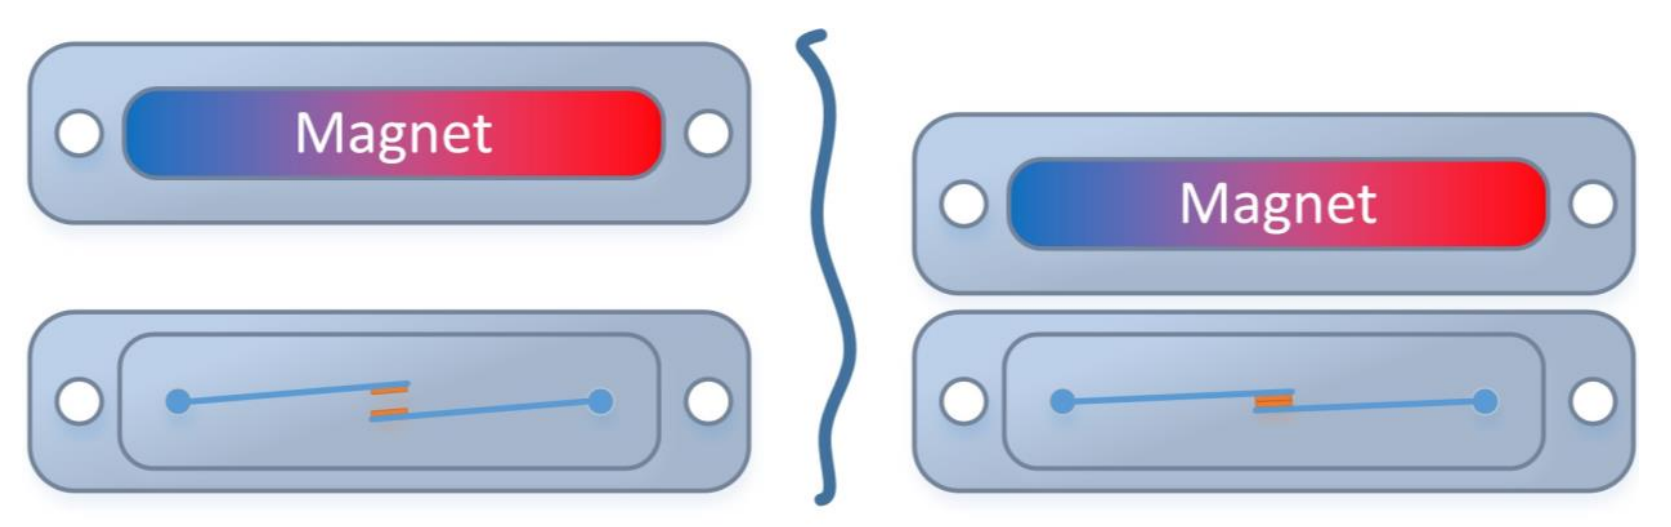
\includegraphics[width=\linewidth]{obrazky-figures/magnetickykontakt.png}
    \caption[Princíp činnosti magnetického kontaktu]{Princíp činnosti magnetického kontaktu\cite{magnetickykontakt}}
    \label{fig:magnetickykontakt}
\end{figure}

\subsubsection{Detektory rozbitia skla}

Keďže najjednoduchším spôsobom ako preniknúť do stráženého objektu je práve cez rozbité okno je dôležité myslieť na ich ochranu. Existuje hneď niekoľko spôsobov ako detekovať rozbitie skla:
\begin{itemize}
    \item \textit{poplachové fólie} - pracujú na princípe vodivých pásikov alebo plôch zaliatych vo vnútri fólie. Poplach je vyvolaný prerušením vodivého pásika. Nalepujú sa na sklenené výplne dverí, okien a výkladov.
    \item \textit{kontaktné snímače} - pracujú na princípe uzavretého elektrického obvodu. Rozbitím skla sa naruší a vyvolá tak poplach. Nedostatkom je nízka odolnosť voči vyrazeniu skla.
    \item \textit{piezoelektrické snímače} - vyhodnocujú otrasy na skle, ktoré vznikajú pri rozbití, rezaní skla. Umiestňujú sa do rohu skla a majú dosah 1,5 až 3 m.
    \item \textit{akustické detektory rozbitia skla} - detekujú zvuk rozbitia skla pomocou mikrofónu. Majú dosah až 10 m od stráženého skla. Sú náchylnejšie na falošné poplachy, ktoré môže vyvolať zvoniaci telefón, rozbitie skla vonku či brzdenie električky.
\end{itemize}

\subsubsection{Pasívne infračervené detektory}\label{sec:pir}

Pasívne infračervené detektory (PIR – Passive Infrared Receiver) snímajú zmeny v~infračervenom pásme elektromagnetického vlnenia vo svojom okolí, na ich základe následne vyhodnocujú narušenie. Využíva sa pyroelektrický senzor, ktorý reaguje na pohybujúce sa teleso s~teplotou odlišnou od teploty okolia. Ten je doplnený o~optický systém, ktorý má funkciu zosilnenia signálu a zvýšenie citlivosti senzora. Využívajú sa Fresnelové šošovky alebo často sústava lomených zrkadiel napríklad tzv. čierne zrkadlo, ktoré neodráža viditeľne svetlo, ale naopak dobre odráža žiarenie vygenerované ľudským telom. PIR detektor je najcitlivejší na pohyb kolmý na optickú os detektora. Tieto detektory sú veľmi populárne najmä vďaka ich pomerne jednoduchej konštrukcii a nízkej cene. Ich výhodou je tiež, že dokážu detekovať prítomnosť človeka bez ožarovania elektromagnetickým vlnením, na ktoré môžu byť ľudia citlivý.\cite{velas_ezs}

V~prípade EZS stupňa 3 a 4 (definované v~tabuľke \ref{tab:stupenzabezpecenia}) musia byť detektory pohybu doplnené aj prostriedkami pre detekciu zakrytia (maskovania).\cite{csn-en-50131-1}

Na trhu sú dostupné detektory s~rôznymi detekčnými charakteristikami (vejár, chodba, záves),
ktorých typ závisí od použitia danej šošovky. Ich detekčné charakteristiky môžeme vidieť na obrázkoch \ref{fig:pir-vejar}, \ref{fig:pir-zaclona}, \ref{fig:pir-chodba} a \ref{fig:pir-strop}. V~ľavej časti môžeme vidieť pohľad zhora a v~pravej časti pohľad zo strany.

\begin{figure}[!ht]
    \centering
    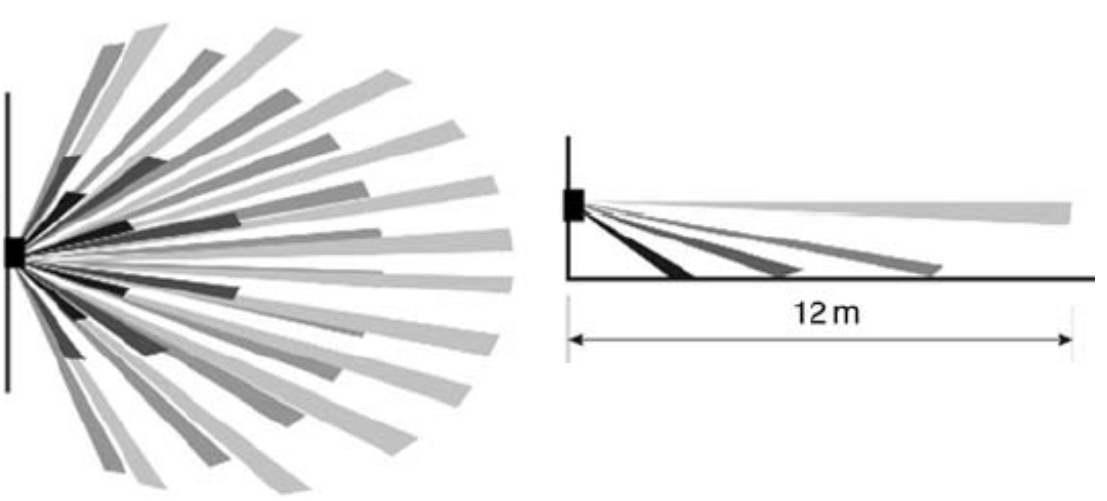
\includegraphics[width=0.75\linewidth]{obrazky-figures/PIR-vejar.png}
    \caption[Detekčná charakteristika PIR typu vejár]{Detekčná charakteristika PIR typu vejár\cite{PIR-vejar}}
    \label{fig:pir-vejar}
\end{figure}

\begin{figure}[!ht]
    \centering
    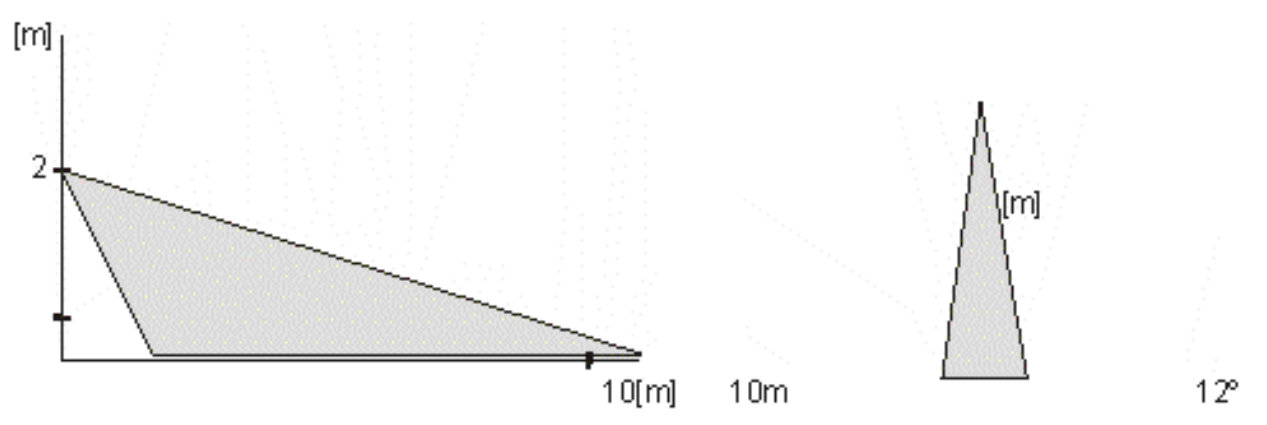
\includegraphics[width=0.75\linewidth]{obrazky-figures/PIR-zaclona.png}
    \caption[Detekčná charakteristika PIR typu záclona]{Detekčná charakteristika PIR typu záclona\cite{velas_ezs}}
    \label{fig:pir-zaclona}
\end{figure}

\begin{figure}[!ht]
    \centering
    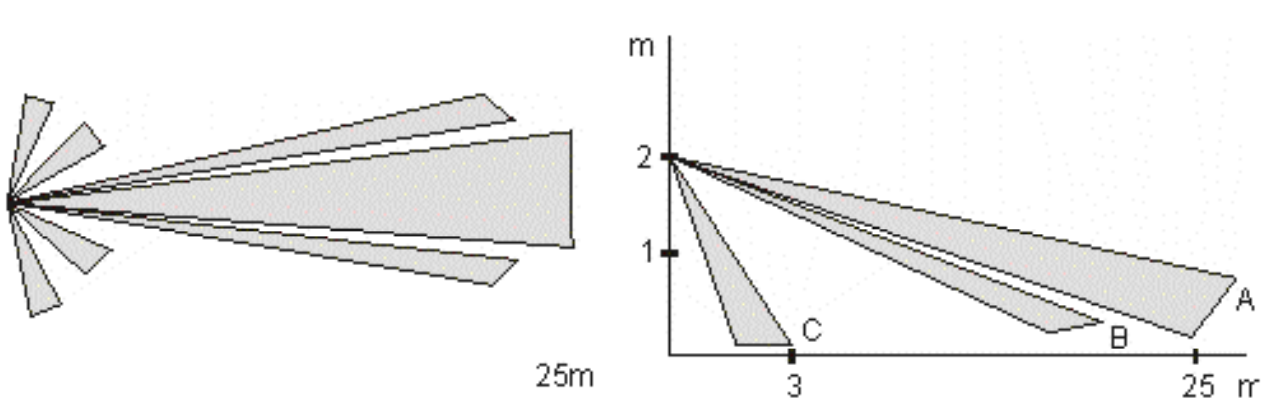
\includegraphics[width=0.75\linewidth]{obrazky-figures/PIR-chodba.png}
    \caption[Detekčná charakteristika PIR typu chodba]{Detekčná charakteristika PIR typu chodba\cite{velas_ezs}}
    \label{fig:pir-chodba}
\end{figure}

\begin{figure}[!ht]
    \centering
    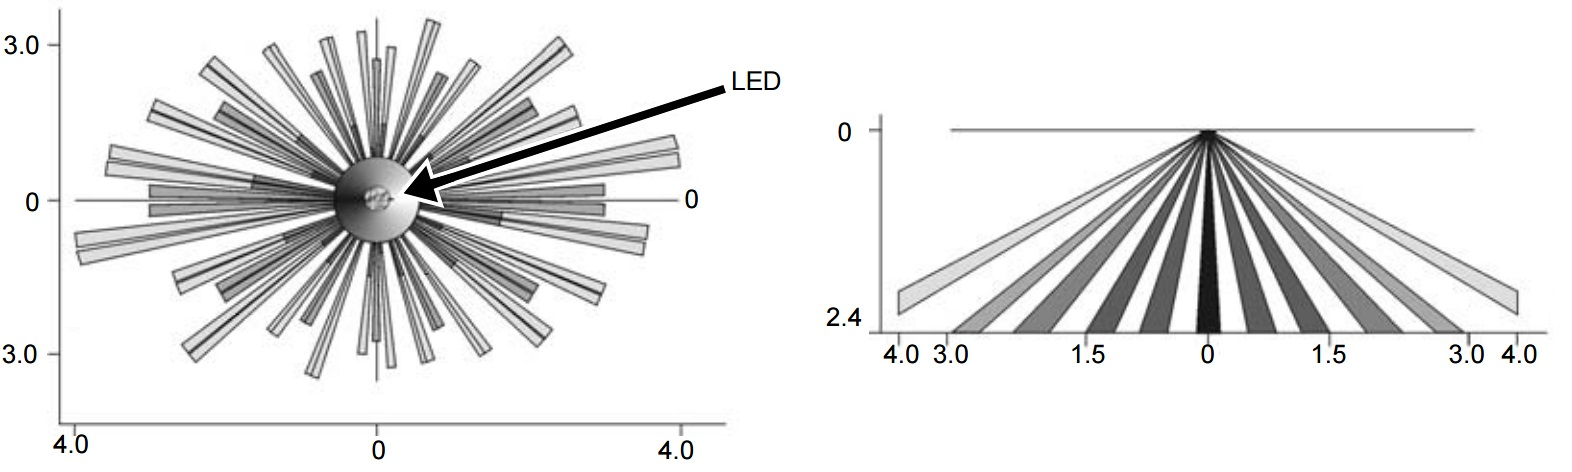
\includegraphics[width=0.75\linewidth]{obrazky-figures/PIR-strop.jpg}
    \caption[Detekčná charakteristika stropného PIR senzora]{Detekčná charakteristika stropného PIR senzora\cite{PIR-strop}}
    \label{fig:pir-strop}
\end{figure}

\subsubsection{Ultrazvukové detektory}

Patria medzi aktívne prvky, teda do priestoru vysielajú energiu. Vysielač vysiela vlnenie konštantnej frekvencie nad pásmom počuteľného zvuku. Následne prijímač prijíma odrazený zvuk a vyhodnocuje fázy, ktoré vznikajú pri pohybe telesa v~chránenom priestore. Jedná sa v~podstate o~aplikáciu Dopplerovho javu v~pásme ultrazvuku. Na ultrazvuk môžu byť citlivé zvieratá (pes, netopier a pod.), ktoré tento zvuk môžu počuť. Dosah detektoru je približne 10 m. Ich citlivosť sa môže znížiť v~prítomnosti materiálov, ktoré pohlcujú zvuk ako koberce, penové materiály a podobne.\cite{Krecek}

\subsubsection{Mikrovlnné detektory}

Vychádzajú z~rovnakého princípu ako ultrazvukové detektory, pracujú však vo frekvenčnom pásme elektromagnetického vlnenia. Taktiež patria medzi aktívne prvky. Ich typický dosah je 15 až 30m. Na rozdiel od ultrazvukových a PIR senzorov sú citlivé na rušenie z~okolia, preto je pravdepodobnosť vzniku falošného poplachu vyššia.\cite{velas_ezs}

\subsubsection{Duálne detektory}

Ide o~spojenie PIR a ultrazvukového, prípadne mikrovlnného detektoru. Myšlienka za spojením je, že je malá pravdepodobnosť súčasného vzniku javov, ktoré by mohli vyvolať falošný poplach pri viacerých čidlách pracujúcich na rozdielnych fyzikálnych princípoch. Zároveň zvyšujú odolnosť voči poruchám. Detektory často umožňujú dve nastavenia - poplach sa spustí pri reakcii oboch čidiel alebo na vyvolanie poplachu stačí ľubovoľný detektor.\cite{velas_ezs}

\subsection{Overovanie spojenia}

Integrita spojenia senzorov s~ústredňou musí byť pravidelne kontrolovaná v~intervaloch špecifikovaných v~tabuľke \ref{tab:interval_overenia}. Stupňom rozumieme stupeň zabezpečenia definovaný v~tabuľke \ref{tab:stupenzabezpecenia} a jednotlivé časy sú maximálne prípustné intervaly medzi signálmi alebo správami komunikácie. V~prípade, že komunikácia nie je v~tomto čase overená, systém by mal vyvolať oznámenie o~poruche, prípadne o~sabotáži. Zároveň systém nesmie byť prepnutý do stavu stráženia, ak nebola komunikácia overená v~intervale podľa tabuľky \ref{tab:interval_overenia}.

\begin{table}[ht]
    \centering
    \renewcommand{\arraystretch}{1.5}
    \begin{tabular}{|c|c|c|c|c|}
        \hline
         & Stupeň 1 & Stupeň 2 & Stupeň 3 & Stupeň 4 \\ \hline
        Periodická komunikácia & 240 min & 120 min & 100 s~& 10 s~\\ \hline
        Nastavovanie stavu stráženia & 60 min & 20 min & 60 s~& 10 s\\ \hline
    \end{tabular}
    \caption[Intervaly overovania]{Intervaly overovania\cite{csn-en-50131-1}}
    \label{tab:interval_overenia}
\end{table}



\subsection{Ovládacie a indikačné zariadenia}

Ovládacie prvky slúžia na uvedenie systému do stavu stráženia alebo do stavu pokoja. Zároveň slúžia aj na zadávanie užívateľských kódov pre ovládanie systému, odstavenie poplachu, základnú správu systému.
\begin{itemize}
    \item \textbf{blokovací zámok} - kombinuje mechanické zabezpečenie vstupných dverí s~ovládaním EZS. Pri odomknutí dverí sa systém automaticky uvedie do stavu odstrážené. Zároveň pri zamykaní sa systém uvedie do stavu zabezpečené. Zámok je pritom možné uzamknúť len ak je EZS v~normálnom stave. Použitie je prirodzené a jednoduché. Ide o~jeden z~najnákladnejších spôsobov ovládania systému.
    \item \textbf{spínací zámok} - podobný blokovaciemu zámku, neobsahuje systém blokovania uzamknutia dverí v~prípade poruchy či chyby obsluhy (napríklad otvorené okno).
    \item \textbf{kódové klávesnice} - je nutné, aby elektronika klávesnice bola umiestnená v~strážených priestoroch. Prináša nevýhodu, že užívateľ si musí zapamätať kód. Ten je však potrebné pravidelne meniť.
    \item \textbf{ovládanie kartou} - výhodou je multifunkčnosť karty, a teda možnosť využiť ju na ďalšie použitie ako obedy, dochádzkový systém, parkovanie a podobne. Nevýhodou je prenosnosť karty, prípadne možnosť jej skopírovania.
    \item \textbf{diaľkové ovládanie} - musí byť chránené vhodným kódom, aby sa nedal zachytiť jeho signál a vyrobiť kópia. Môže byť doplnené aj o~ďalšie funkcie ako spustenie tiesňového hlásenia a pod.\cite{velas_ezs}
\end{itemize}

Indikačné prvky informujú o~stave systému napríklad pomocou LED diódy, akustickej, vizuálnej signalizácie, prípadne ich kombináciou. Medzi najbežnejšie hlásenia patria:
\begin{itemize}
    \item stav pokoja/stráženia
    \item uvádzanie do stavu stráženia
    \item hlásenie poruchy
    \item poplach
\end{itemize}

Akustické výstražné zariadenie musí byť v~prevádzke aspoň 90 sekúnd pričom maximálna doba jeho činnosti nesmie prekročiť 15 minút.\cite{csn-en-50131-1}

Systém môže byť doplnený o~ďalšie doplnkové zariadenia, ktoré slúžia na komunikáciu s~pultom centrálnej ochrany alebo na komunikáciu s~majiteľom.\cite{Krecek}


\chapter{Bluetooth Low Energy}

Bluetooth je technológia na bezdrôtovú komunikáciu medzi dvoma a viacerými zariadeniami. Má široké využitie od rôznych ovládačov, cez prehrávanie hudby až po prenos súborov medzi zariadeniami. Operuje v~rovnakom frekvenčnom pásme ako technológia Wi-Fi - 2,4 GHz. Vďaka tomu môžu menšie zariadenia využívajúce obe technológie súčasne používať spoločnú anténu, to však prináša aj nevýhodu v~podobe rušenia.

Bluetooth Low Energy (BLE) je navrhované pre nízkoenergetickú operáciu. Od Bluetooth verzie 4.0 je súčasťou štandardu. Je primárne učené na výmenu kratších informácií nižšou rýchlosťou. Tento štandard je často využívaný pri zaradeniach napájaných z~batérie, ako sú napríklad zariadenia Internetu vecí (IoT). Zariadenia s~podporou tejto technológie sú označované často ako \textit{Bluetooth Smart}, respektíve \textit{Bluetooth Smart Ready} pre zariadenia spájajúce BLE a klasické Bluetooth.

\section{Porovnanie s~klasickým Bluetooth}

Obe technológie využívajú rovnaké frekvenčné pásmo 2,402 - 2,480 GHz. Využívajú však rozdielny počet a rozostupy kanálov. BLE obsahuje 40 kanálov s~rozostupom 2 MHz. Z~toho sú 3 kanály určené na prenos informácií o~zariadení tzv. \textit{advertising}, zvyšných 37 kanálov je určených na prenos dát. V~prípade klasického Bluetooth je týchto kanálov 79 a s~rozostupom 1 MHz. V~závislosti na použitej fyzickej vrstve protokol BLE dosahuje rýchlosť až 2 Mb/s (Bluetooth v5.0), oproti tomu klasické Bluetooth dosahuje rýchlosť až 3 Mb/s. BLE je v~závislosti na použití 2 až 100 krát menej náročné na spotrebu energie.
\cite{bluetooth}

\section{Topológia}
Bluetooth Low Energy dokáže pracovať s~tromi rôznymi topológiami siete:
\begin{itemize}
    \item \textbf{Point-to-point} - komunikácia medzi dvomi zariadeniami (1:1), je podporovaná ako pre BLE tak aj pre Bluetooth. Využíva sa napríklad na prehrávanie hudby. Táto topológia je vhodná pre rôzne typy zariadení. V~prípade BLE sa táto topológia využíva napríklad pre fitnes zariadenia, merače tepu, periférie a príslušenstvo pre počítač.
    \item \textbf{Broadcast} - jedno zariadenie komunikuje s~viacerými zariadeniami (1:M). Táto topológia je podporovaná len v~BLE, využíva sa napríklad na lokalizáciu a navigáciu vo vnútri budovy.  
    \item \textbf{Mesh} - komunikácia viacerých zariadení (M:N), je podporovaná len pre BLE. Vďaka tejto topológii je možné vytvoriť veľkú sieť zariadení. Táto topológia je vhodná ak je potrebné spojiť desiatky, stovky či tisícky zariadení, ktoré potrebujú medzi sebou spoľahlivo a bezpečne komunikovať. Využitie má napríklad v~monitorovaní alebo automatizácii.\cite{bluetooth}
\end{itemize}

\section{Architektúra} \label{sec:arch}
Bluetooth implementuje kompletnú architektúru od fyzickej komunikácie medzi zariadeniami až po komunikáciu s~vlastnými aplikáciami. Bluetooth je teda takzvaný \textit{full protocol stack}. Kompletnú architektúru môžeme vidieť na obrázku \ref{fig:ble_stack}.

\begin{figure}[ht]
    \centering
    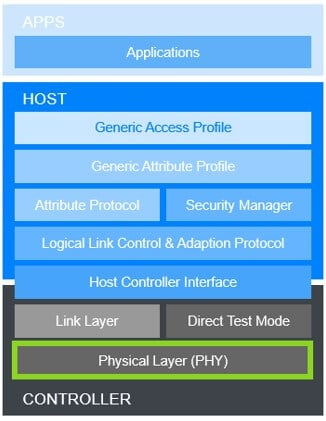
\includegraphics[scale=0.6]{obrazky-figures/bluetooth_le_protocol_stack.jpg}
    \caption[Architektúra BLE]{Architektúra BLE\cite{bluetooth}}
    \label{fig:ble_stack}
\end{figure}

\begin{itemize}
    \item \textbf{Physical Layer (PHY)} - fyzická vrstva, prenáša samotný analógový signál a transformuje ho na digitálny. Od Bluetooth v5.0 rozlišujeme 3 varianty PHY. Sú to:
    \begin{itemize}
        \item LE 1M - rýchlosť prenosu dát 1~Mb/s, pôvodná PHY definovaná v~Bluetooth v4.0, chyby dokáže detekovať, ale nie opraviť
        \item LE 2M - rýchlosť 2~Mb/s, vzdialenosť prenosu je oproti LE 1M zmenšená na približne 80~\%, chyby dokáže detekovať, ale nie opraviť
        \item LE Coded - dokáže teoreticky zvýšiť vzdialenosť prenosu dvoj až štvornásobne, a to pomocou redundancie dát v~odosielanom pakete. Vďaka tomu zariadenie na druhej strane dokáže detekovať a opraviť chyby v~dátach. Existujú dva varianty v~závislosti na úrovni redundancie - S=2 a S=8, kde S~udáva počet redundantných dát v~odosielanom pakete. To ma však nepriaznivý vplyv na rýchlosť odosielania, ktorá je znížená na 500~Kb/s, respektíve pre S=8 na 125~Kb/s. 
    \end{itemize}
    \item \textbf{Link Layer} - linková vrstva, jej úlohou je skenovanie, spravuje, vytvára spojenia
    \item \textbf{Direct Test Mode} - umožňuje testovanie fyzickej vrstvy
    \item \textbf{Host Controller Interface (HCI)} - sprostredkúva komunikáciu medzi vrstvami, môže využívať API alebo aj iné štandardné rozhrania ako USB, UART, SPI. 
    \item \textbf{Logical Link Control and Adaption protocol (L2CAP)} - zapuzdruje dáta pre ďalšie vrstvy
    \item \textbf{Attribute Protocol} - samotné zdieľané dáta
    \item \textbf{Security Manager} - zabezpečuje párovanie a distribúciu kľúčov
    \item \textbf{Generic Attribute Profile (GATT)}
    \item \textbf{Generic Access Profile (GAP)} - priama komunikácia s~aplikáciou, zabezpečuje pripojenia na služby pre BLE zariadenie
    \cite{bluetooth}\cite{ble-arch}
\end{itemize}
Bližšie sa k~GAP a GATT venujem v~nasledujúcich podkapitolách \ref{sec:gap} a \ref{sec:gatt}.

\section{Rozsah pokrytia}

Rozsah pokrytia Bluetooth je závislý na viacerých faktoroch. Teoreticky je možné dosiahnuť vzdialenosť od metra až cez jeden kilometer. Bluetooth je navrhované na podporu rôznych rozsahov, konkrétna implementácia je ponechaná na vývojároch, aby si vybrali vhodné riešenie pre ich potreby. Jedným z~faktorov je výber fyzickej vrstvy (PHY), kde rozdiely boli spomínané už v~podkapitole \ref{sec:arch}. Ďalšími faktormi sú senzitivita prijímača, vysielací výkon, dosah antény alebo strata signálu po ceste, napríklad vďaka prekážkam a podobne.\cite{bluetooth}

\section{Generic Access Profile (GAP)}\label{sec:gap}

Ide o~základný profil, ktorý implementujú všetky Bluetooth zariadenia. Definuje základné požiadavky zariadenia. Vyskytuje sa ako v~klasickej (BR/EDR) verzii tak aj v~Low Energy. Pre BLE definuje jednotlivé vrstvy architektúry, správanie a metódy pre vyhľadanie zariadenia, pripojenie k~nemu, bezpečnosť a podobne.
Zároveň definuje 4 špecifické roly, pričom zariadenie môže podporovať viacero rolí súčasne. Každá z~rolí je optimalizovaná na špecifické použitie. Sú to:
\begin{itemize}
    \item \textbf{Broadcaster} - vysielanie dát, nepodporuje spojenia
    \item \textbf{Observer} - prijímanie dát, komplementárny k~Broadcaster, nepodporuje spojenia
    \item \textbf{Peripheral} - podporuje jedno spojenie, menej komplexné ako Central
    \item \textbf{Central} - podporuje niekoľko spojení\cite{bluetooth}
\end{itemize}

\section{Attribute Protocol}

Umožňuje čítať a zapisovať malé dáta na server. Každá hodnota, typicky pár bajtov, sa nazýva atribút (attribute). Tento protokol definuje pre každú hodnotu univerzálnu unikátnu identifikáciu~-~UUID. Tie môžu mať dĺžku 16, 32 alebo 128 bitov.
Protokol definuje dve roly~-~klient a server. Zariadenie dokáže zároveň fungovať ako server aj ako klient. Server ukladá dáta a akceptuje požiadavky, príkazy a potvrdenia od klienta. Taktiež odosiela odpovede a upozornenia pri výskyte špecifikovanej udalosti na serveri.\cite{bluetooth}

\subsection{Generic Attribute Profile (GATT)}\label{sec:gatt}

GATT definuje hierarchickú štruktúru dát. Je postavený na Attribute profile, definuje operácie nad dátami uloženými a zasielanými pomocou neho. taktiež špecifikuje formát dát, ktoré sa nachádzajú na serveri, sú formátované ako služby (services) a charakteristiky (characteristics). Jedna služba môže obsahovať niekoľko charakteristík. Služby môžu byť aj zanorené, pričom zanorená služba existuje aj samostatne aj v~rámci nadradenej služby. Charakteristiky obsahujú jednu hodnotu, jej vlastnosti a môžu obsahovať aj niekoľko deskriptorov, ktoré opisujú hodnotu. Na obrázku \ref{fig:gatt} je možné vidieť ako by napríklad mohla vyzerať hierarchia GATT.\cite{bluetooth}

\begin{figure}[ht]
    \centering
    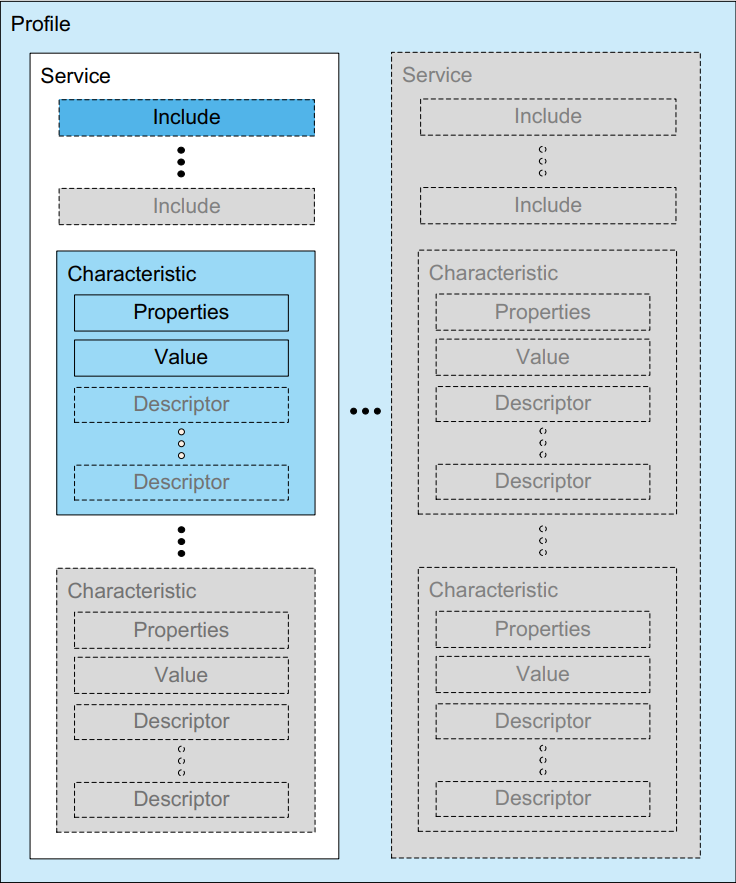
\includegraphics[scale=0.4]{obrazky-figures/gatt.png}
    \caption[Profilová hierarchia založená na GATT]{Profilová hierarchia založená na GATT\cite{bluetooth}}
    \label{fig:gatt}
\end{figure}


\section{Párovanie zariadení}

Pri BLE môžeme rozlišovať dva spôsoby spojenia zariadení a výmeny kľúčov. V~prípade, že ide o~dočasné kľúče a krátkodobé tzv. \textit{párovanie}, je spojenie len dočasné a je nutné pri každom párovaní znova vymeniť nové dočasné kľúče. V~prípade viazania alebo presnejšie \textit{bonding} si zariadenia uložia dlhodobé kľúče do internej pamäte. Vďaka tomu dokážu šifrovať komunikáciu, overovať podpísané dáta a rozšifrovať náhodne generované adresy.
Proces viazania (bonding) zariadení môžeme rozdeliť na 3 fázy. Tento proces môžeme pre názornosť lepšie vidieť na obrázku \ref{fig:bonding}. V~prípade párovania je postup rovnaký, ale končí sa fázou 2. Tieto fázy sú:
\begin{itemize}
    \item fáza 1 - výmena informácii o~podporovaných vstupoch a výstupoch (napríklad obrazovka a klávesnica, tie sú využité pre zadanie alebo zobrazenie dočasného kľúča), možnostiach zabezpečenia ako ochrana proti odchytávaniu komunikácie alebo tzv. \textit{Man-In-The-Middle} útoku. Nasleduje výmena párovacej informácie medzi zariadeniami. Okrem iného je v~týchto paketoch znak definujúci, či sa jedná len o~párovanie alebo následne aj bonding.
    \item fáza 2 - nasleduje výmena dočasných kľúčov pre šifrovanie komunikácie. Existuje niekoľko spôsobov výmeny týchto kľúčov. Časté je generovanie 6 miestneho kódu na jednej strane a prepísanie na druhej. Ďalšie spôsoby sú porovnávanie kódov, jednoduché potvrdenie tlačidlom alebo využitie inej technológie na distribúciu kľúča (napr. NFC). Pokračuje sa overením kľúčov. V~prípade párovania nasleduje odosielanie samotných dát.
    \item fáza 3 - Táto časť komunikácie je už šifrovaná kľúčmi vygenerovanými vo fáze 2. Nasleduje generovanie a výmena dlhodobých kľúčov a výmena samotných dát. Pri ďalšom pripojení tento proces nie je potrebné opakovať.\cite{bluetooth}
\end{itemize}

\begin{figure}[ht]
    \centering
    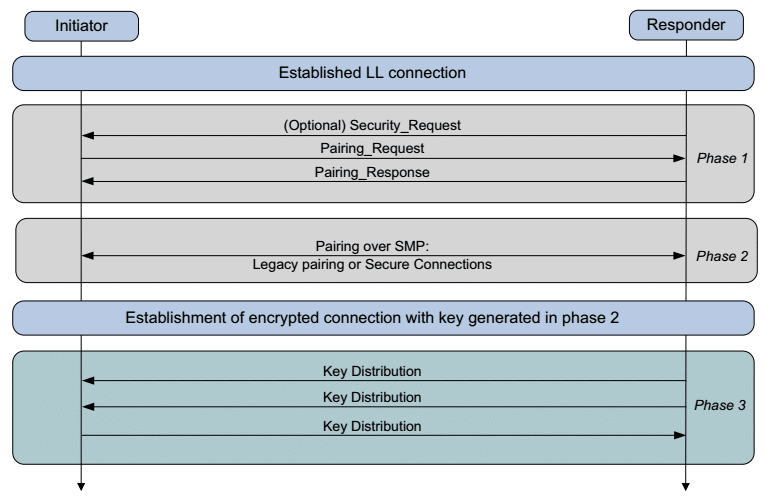
\includegraphics[width=0.75\linewidth]{obrazky-figures/pairing-flowchart.png}
    \caption[Bonding diagram komunikácie]{Bonding diagram komunikácie\cite{bluetooth}}
    \label{fig:bonding}
\end{figure}



\chapter{ESP32}

ESP32 je populárna séria systémov na čipe (SoC - System on chip) od spoločnosti Espressif Systems, ktorá vznikla v~roku 2016. Je nasledovníkom známeho ESP2866. Ide o~výkonnejší modul, ktorý má veľa ďalších vlastností ako podporu Bluetooth, viac univerzállnych vstupno-výstupných (GPIO) pinov a podobne. V~závislosti na variante existujú rôzne výkonné modely s~rôznymi vlastnosťami.
Vďaka jeho pomerne nízkej cene a nízkej spotrebe je vhodný na automatizáciu domácnosti, v~IoT zariadeniach, v~medicíne, priemysle a podobne. Bol navrhnutý ako samostatne fungujúci mikrokontrolér s~ohľadom na maximálny výkon s~minimálnou spotrebou energie.

\section{Architektúra}

\begin{figure}[ht]
    \centering
    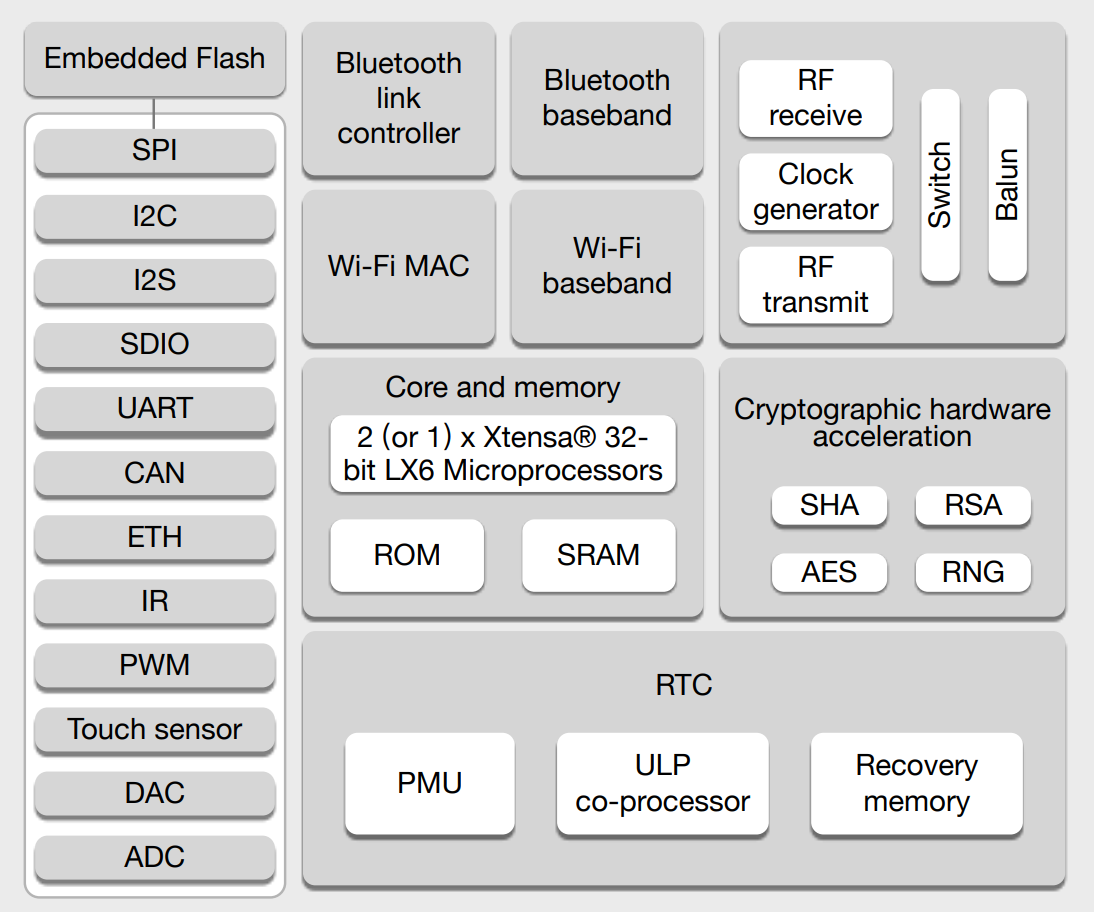
\includegraphics[scale=0.3]{obrazky-figures/esp32_diagram.png}
    \caption[Funkčný blokový diagram ESP32]{Funkčný blokový diagram ESP32\cite{esp-datasheet}}
    \label{fig:esp_diagram}
\end{figure}

Jadrom ESP32 je 32-bitový procesor Xtensa s~jedným alebo dvomi jadrami a frekvenciou až 240Mhz, ten je doplnený o~520~KB SRAM a 448~KB ROM. Zároveň na čipe môžeme nájsť podporu aj pre Wi-Fi 2,4~Ghz (802.11~b/g/n), Bluetooth v4.2 BR/EDR aj BLE (podľa aktuálnych informácií bol certifikovaný aj na v5.0\footnote{\url{https://www.espressif.com/en/news/BLE_5.0_Certification}}).
Čip má podporu aj pre hardvérovú akceleráciu šifrovania, množstvo rôznych periférií a 34 vstupno-výstupných portov (GPIO). Celý blokový diagram je znázornený na obrázku \ref{fig:esp_diagram}.\cite{esp-datasheet}


\section{Varianty}

ESP32 je dostupné v~niekoľkých verziách. Tie môžeme v~základe rozdeliť na SoC, moduly a vývojové dosky, viď obrázok \ref{fig:esp32_varianty}. Tie sa ďalej rozdeľujú napríklad podľa špecifikácií a dostupných súčastí. Súčasťou  modulov a vývojových dosiek býva často aj anténa vytlačená priamo na doske, prípadne je možnosť pripojenia externej antény, ktorou sa dokáže zväčšiť dosah zariadenia. Existujú rôzne varianty vývojových modulov, často môžme nájsť varianty s~pridanou funkcionalitou ako je napríklad kamera, čítačka microSD kariet a podobne.

\begin{figure}[ht]
    \centering
    \begin{subfigure}{.3\textwidth}
      \centering
      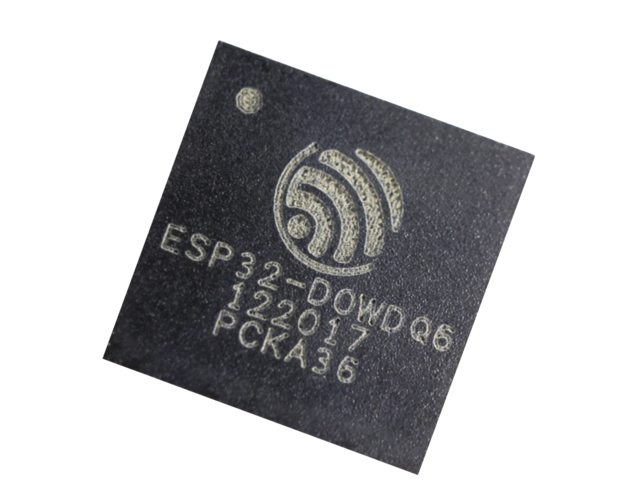
\includegraphics[width=.8\linewidth]{obrazky-figures/esp-soc.png}  
      \caption{SoC\footnotemark[2]}
      %https://www.gridconnect.com/products/esp32-d0wdq6-2-4-ghz-wi-fi-bluetooth-combo-chip
      \label{fig:esp32_soc}
    \end{subfigure}
    \begin{subfigure}{.3\textwidth}
      \centering
      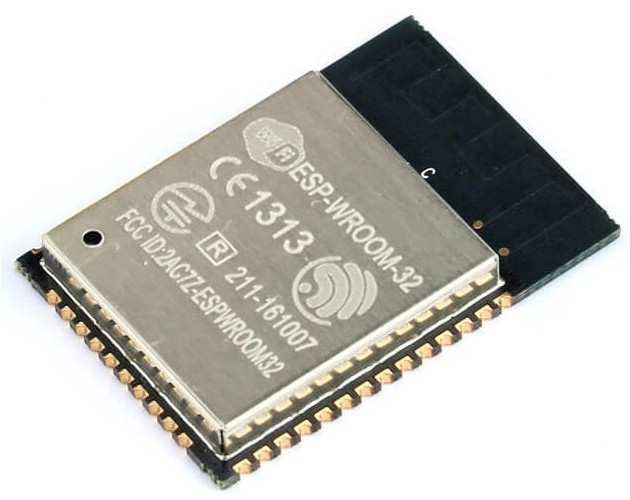
\includegraphics[width=.8\linewidth]{obrazky-figures/esp-module.jpg}  
      \caption{Modul\footnotemark[3]}
      %https://www.blueberrye.me/compute-boards/esp-wroom-32-esp32-wifi-bt-ble-mcu-module/a-1690130
      \label{fig:esp32_module}
    \end{subfigure}
    \begin{subfigure}{.3\textwidth}
      \centering
      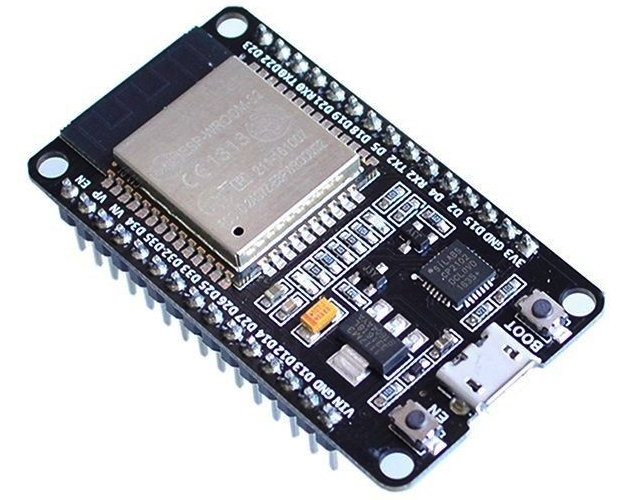
\includegraphics[width=.8\linewidth]{obrazky-figures/esp-dev.png}
      \caption{Vývojová doska\footnotemark[4]}
      %https://navody.arduino-shop.cz/navody-k-produktum/vyvojova-deska-esp32.html
      \label{fig:esp32_dev}
    \end{subfigure}
    \caption{Varianty ESP32}
    \label{fig:esp32_varianty}
\end{figure}

\footnotetext[2]{prevzaté z: \url{https://www.gridconnect.com/products/esp32-d0wdq6-2-4-ghz-wi-fi-bluetooth-combo-chip}}
\footnotetext[3]{prevzaté z: \url{https://www.blueberrye.me/compute-boards/esp-wroom-32-esp32-wifi-bt-ble-mcu-module/a-1690130}}
\footnotetext[4]{prevzaté z: \url{https://navody.arduino-shop.cz/navody-k-produktum/vyvojova-deska-esp32.html}}

\section{Programovanie}

Existuje viacero možností programovania ESP32. Asi najznámejším a najpoužívanejším je Arduino IDE, prípadne editor s~rozšírením PlatformIO. Obe možnosti využívajú pre programovanie jazyk C++. Ide o~riešenie s~jednoduchou inštaláciou, ktoré ponúka menej možností a väčšie výsledné programy. Na základné aplikácie je často postačujúce. Knižnica je aktualizovaná menej často, čo môže priniesť niekoľko problémov.

Ďalšou z~možností je využite frameworku ESP-IDF, ktorý v~podstate rieši všetky problémy spomínané v~knižnici pre Arduino IDE. Prináša však malú nevýhodu programovania v~C a zložitejšiu inštaláciu. Tento nástroj je vyvíjaný samotnou spoločnosťou Espressif Systems a je označovaný za preferovanú formu programovania mikrokontroléru. Je založený na operačnom systéme reálneho času (RTOS), konkrétne na FreeRTOS s~otvoreným kódom.

Jednou z~možností je aj použitie MicroPython, ktorý je založený na Pythone 3.4 a prináša teda výhody vyššieho programovacieho jazyka. Ide o~menej bežný spôsob, a teda existuje na neho menej príkladov a návodov. Zostavenie je založené na frameworku ESP-IDF. Oproti predchádzajúcemu spôsobu ponúka menšie možnosti konfigurácie a menej časté aktualizácie knižnice.

\section{Režim spánku}\label{sec:esp-sleep}

ESP32 podporuje niekoľko režimov spánku čo pomáha ešte viac zmenšovať jeho spotrebu. V~tabuľke \ref{tab:spotreba_esp} je možné vidieť porovnanie jednotlivých módov šetrenia energie. V~poslednom stĺpci tabuľky sú uvedené len pridané časti, takže pre aktuálny riadok platí to isté čo pre predchádzajúci plus naviac informácie v~tomto riadku.

Ako prvý je pre porovnanie uvedený aktívny mód, a teda základný mód so všetkými aktívnymi časťami. V~prípade súčasného využitia Wi-Fi a Bluetooth môže spotreba dosahovať v~špičke až 790~mAh. Pri móde s~uspatým modemom (modem sleep) sú neaktívne Wi-Fi, Bluetooth, rádio vysielač a periférie. Je možné nastaviť frekvenciu procesora a upraviť tak spotrebu. V~ľahkom spánku (light sleep) je naviac pozastavený procesor, dochádza k~uloženiu obsahu RAM. Pri prebudení sa systém vráti do predchádzajúceho stavu. V~hlbokom spánku (deep sleep) je procesor úplne vypnutý, koprocesor stále sleduje zmeny na senzoroch a prebúdza procesor. Narozdiel od ľahkého spánku nedochádza k~automatickej obnove pamäti RAM. Stále je však možné využiť RTC pamäť na uloženie a znovu načítanie dát pri prebudení. Pri hibernácii (hibernation) je naviac odstavený aj koprocesor a RTC pamäť. Všetko okrem jedného časovača a niektorých vstupných RTC je vypnuté. Tie sú zodpovedné za prebudenie systému.\cite{esp-sleep}

\begin{table}[ht]
    \centering
    \renewcommand{\arraystretch}{1.5}
    \begin{tabular}{|c|c|c|}
        \hline
        Mód & Spotreba & Pridané neaktívne časti \\ \hline
        Active & 80~-~260 mA\footnotemark[5] & - \\ \hline
        Modem sleep & 3~-~20 mA & Wi-Fi, Bluetooth, periférie, vysielač\\ \hline
        Light sleep & 0,8 mA & pozastavený procesor\\ \hline
        Deep sleep & 10 $\mu$A & procesor\\ \hline
        Hibernation & 2.5 $\mu$A & koprocesor\\ \hline
    \end{tabular}
    \caption[Porovnanie spotreby v~jednotlivých módoch]{Porovnanie spotreby v~jednotlivých módoch\cite{esp-sleep}}
    \label{tab:spotreba_esp}
\end{table}
\footnotetext[5]{V prípade zasielania dát pomocou Wi-Fi alebo Bluetooth je spotreba vyššia ako pri prijímaní}



\chapter{Mobilné aplikácie}

Existuje niekoľko spôsobov ako vytvoriť aplikácie pre mobilné zariadenia. Základným spôsobom je vývoj natívnych aplikácií. V~súčasnosti je však čoraz častejšie využitie webových technológií ako je HTML, CSS a Javascript. Každá varianta prináša určité výhody a nevýhody, je nutné vybrať technológiu vhodnú pre aktuálne potreby. V~texte sa ďalej primárne zameriam na dva najpopulárnejšie mobilné operačné systémy - Android a iOS.

\section{Natívne aplikácie}

Natívne aplikácie sú aplikácie vyvíjané pre konkrétnu platformu natívnym programovacím jazykom. V~prípade Androidu je to teda Java alebo Kotlin, pre iOS to sú Swift alebo Objective-C. Aplikácie môžu mať prístup k~všetkým senzorom telefónu, ku kontaktom a podobne. Takéto aplikácie sú často plynulejšie a rýchlejšie. Prinášajú však aj nevýhody v~podobe zložitejšieho programovania užívateľského rozhrania. Ďalšou nevýhodou natívnych aplikácií je že sú určené len pre jednu platformu. Aplikácia vytvorená pre iOS nie je podporovaná na zariadeniach s~Androidom a naopak.\cite{hybrid-app}

Existujú však aj frameworky, vďaka ktorým je možné vytvárať multiplatformové natívne aplikácie. Sem patrí napríklad Xamarin, Titanium alebo React Native. Medzi platformami sú minimálne rozdiely a je možné zdieľať až 90~\% kódu. Prispieva to tak k~šetreniu času a tým aj nákladov pri vývoji aplikácie pre obe platformy.\cite{crossplatform-app}

\section{Webové aplikácie}

Ide o~tradičné webové aplikácie, ktoré sú zobrazované pomocou užívateľom zvoleného prehliadača. Majú pomerne obmedzený prístup k~zdrojom zariadenia ako sú senzory a podobne. Aplikácie sa vytvárajú pomocou webových technológií ako je HTML, CSS a Javascript. Tieto technológie môžu byť rozšírené o~ďalšie knižnice a frameworky ako sú Angular, React, Vue a ďalšie. Na funkčnosť aplikácie je pri tom nevyhnutné pripojenie na internet. Vďaka konceptu progresívnych webových aplikácií (Progressive Web Applications) dokážu tieto aplikácie využívať niektoré funkcie známe z~natívnych aplikácií ako napríklad zasielanie upozornení a ďalšie. Výhodou je, že aplikácia nie je uložená priamo v~zariadení a teda nezaberá užívateľovi miesto v~pamäti. Zároveň tento spôsob ponúka okamžité aktualizácie.\cite{hybrid-app} 

\section{Hybridné aplikácie}

Ide o~spojenie natívnych a webových aplikácií. Takto vytvorené aplikácie sú priamo nainštalované v~zariadení, nevyžadujú teda pripojenie na internet. Ide v~podstate o~natívnu aplikáciu s~webovým oknom, v~ktorom je zobrazený samotný obsah. Pre koncového užívateľa je toto webové okno v~podstate neviditeľné a nevidí rozdiel oproti natívnej aplikácii. Ide o~prenosný spôsob programovania aplikácií, jedným kódom je možné vytvoriť multiplatformovú aplikáciu. Výsledná aplikácia môže byť pomalšia oproti natívnej práve vďaka ďalšej vrstve v~aplikácii. Tieto aplikácie sa však stále zlepšujú a rýchlosť oproti natívnym aplikáciam prestáva byť citeľná. Táto technológia je primárne používaná na jednoduchšie aplikácie.\cite{hybrid-app} 

Existuje množstvo frameworkov, ktoré umožňujú takto zabaliť webovú aplikáciu do natívnej. Tie často definujú vlastné prvky užívateľského rozhrania a urýchľujú tak prácu vývojárom. Zároveň to umožňuje zdieľať dizajn jednotlivých prvkov s~užívateľským rozhraním celého systému. Viacero frameworkov je založených na Apache Cordova. Ten poskytuje otvorený kód a vďaka tomu aj možnosť pridávania rozšírení na podporu napríklad Bluetooth, ale aj ďalších senzorov v~zariadení. Samotná aplikácia je vyvíjaná v~HTML, CSS a Javascript. Z~tohto frameworku vychádzajú ďalšie ako je napríklad PhoneGap, Ionic alebo Framework7, ktoré umožňujú využívať ďalšie knižnice. Rozdiely medzi týmito frameworkami sú však pre užívateľa minimálne a výber je často na preferenciách podporovaných knižníc a podobne.\cite{crossplatform-app}


\chapter{Návrh prototypu}

Cieľom práce je navrhnúť zabezpečovacie zariadenie, ktoré bude schopné detekovať prítomnosť majiteľa pomocou BLE. Toto elektronické zabezpečovacie zariadenie bude primárne určené pre bežné domácnosti. Pôjde teda o~systéme so stupňom zabezpečenia 2, podľa tabuľky \ref{tab:stupenzabezpecenia}. Výsledné zariadenie musí obsahovať BLE modul, pomocou ktorého bude pravidelne skenovať okolie pre prítomnosť známych zariadení. O~skenovanie sa pritom bude starať samotná ústredňa zabezpečovacieho zariadenia, ktorá zároveň vyhodnocuje informácie zo senzorov. Na základe toho sa systém dokáže prepínať medzi rôznymi stavmi (odstrážené, zabezpečené, alarm a podobne).

Existuje niekoľko spôsobov ako takýto systém vytvoriť. Jedným zo spôsobov je napríklad využite topológie \textit{Mesh}. Pomocou nej je možné spojiť zariadenia do jednej veľkej siete. Takýto systém disponuje pomerne veľkým dosahom vďaka spôsobu komunikácie. Jeho nevýhodou je, že zariadenia nie je možné uviesť do hlbokého spánku. Tento spôsob by teda vyžadoval napájanie jednotlivých senzorov z~elektrickej siete, prípadne by znamenal pomerne časté vymieňanie batérií. V~prípade zabezpečovacieho systému by to vytvorilo nepohodlnú údržbu, respektíve inštaláciu systému. Senzory sú totiž často umiestňované na miesta, kde nie je v~dosahu elektrická zásuvka.

Druhým navrhovaným spôsobom je využitie topológie \textit{Point-to-point}. V~tomto prípade ústredňa funguje ako server a senzory sa na ústredňu pripájajú ako klienti. Keďže klient (senzor) iniciuje spojenie, udržiava sa v~aktívnom stave čo najkratší čas. Tým sa šetrí spotrebovaná energia a senzor dokáže fungovať aj z~batérie. Po skončení komunikácie je možné senzor uspať na zvolenú dobu. V~prípade zaznamenania narušenia je senzor prebudený zo spánku a odošle hlásenie na hlavnú jednotku. Tento spôsob komunikácie sa ukázal ako vhodnejší pre navrhovaný systém, a teda celá nasledujúca kapitola popisuje detailnejšie túto variantu.

Pre začiatok je nutné definovať pojmy. V~systéme sa vyskytujú dva druhy BLE zariadení~-~senzory a užívateľom definované zariadenia. V~nasledujúcom texte budú BLE zariadeniami myslené len zariadenia, ktoré užívateľ definoval ako zariadenia prepínajúce systém do stavu odstrážené. Pre senzory je často využívaný aj presnejší pojem jednotka so senzorom.

Celý navrhovaný systém môžeme vidieť ako blokový diagram na obrázku \ref{fig:navrh_diagram}. Súčasťou diagramu sú obe časti systému - ústredňa aj samotné senzory. Podrobnejšie sa k~jednotlivým častiam venujem v~nasledujúcich kapitolách.

\begin{figure}[ht]
    \centering
    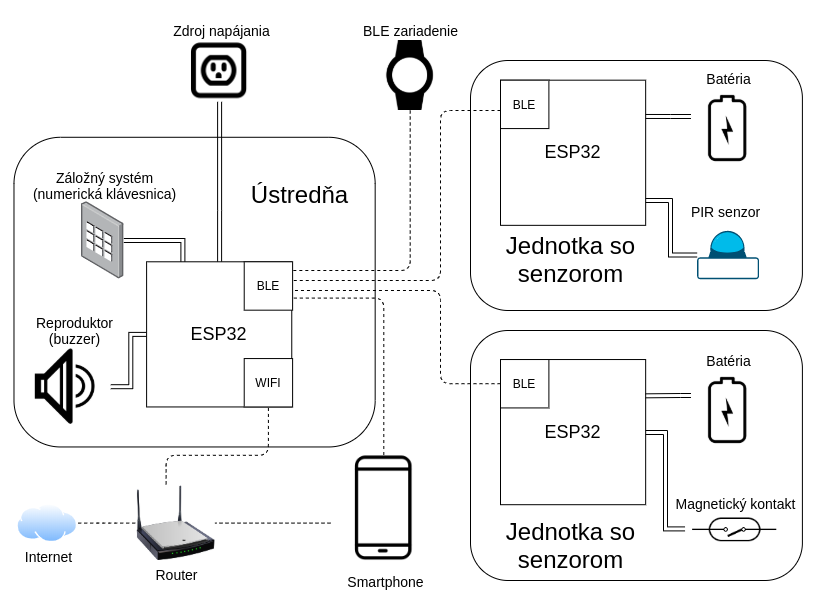
\includegraphics[scale=0.4]{obrazky-figures/block_diagram.png}
    \caption{Blokový diagram prototypu}
    \label{fig:navrh_diagram}
\end{figure}

\section{Stavy systému}

Zariadenie musí byť schopné rozlišovať rôzne stavy stráženia a prepínať medzi nimi. Na obrázku \ref{fig:state_diagram} je zobrazený stavový diagram, ktorý ukazuje jednotlivé stavy a prechody medzi nimi.

\begin{figure}[!ht]
    \centering
    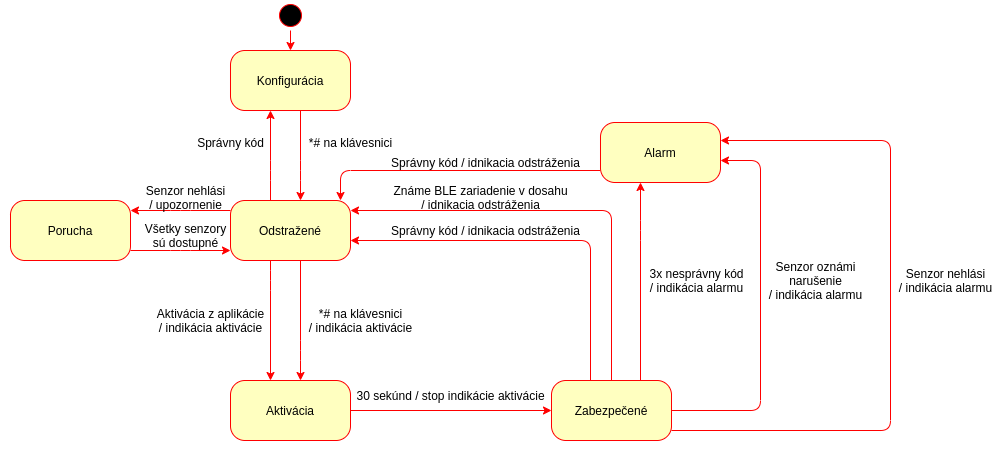
\includegraphics[width=\linewidth]{obrazky-figures/state_diagram.png}
    \caption{Stavový diagram prototypu}
    \label{fig:state_diagram}
\end{figure}

\noindent Navrhované stavy zahrňujú:

\begin{itemize}
    \item \textbf{konfigurácia} - stav určený pre konfiguráciu samotného systému. V~tomto stave je možné zmeniť kód, ktorým sa zariadenia dokáže prepnúť zo stavu zabezpečené naspäť do stavu \textit{odstrážené}. Zároveň je možné zmeniť známe zariadenia, nastavenia Wi-Fi siete a podobne. Okrem tohto stavu nie je možné meniť nastavenia systému. Systém je v~tomto stave možné meniť z~akéhokoľvek zariadenia v~lokálnej sieti. Na to aby sa systém do tohto stavu dostal je potrebné zadať správny kód na číselnej klávesnici.
    \item \textbf{odstrážené} - režim, v~ktorom je systém pripravený kedykoľvek na prepnutie do stavu aktivácie systému. V~tomto režime sa kontrolujú pripojené senzory, nie však ich výstup, ale len ich dostupnosť. Zadaním správneho kódu je možné prepnúť ústredňu do stavu konfigurácie.
    \item \textbf{porucha} - nastane v~prípade nedostupnosti aspoň jedného senzoru. Systém v~tomto stave nie je možné aktivovať. Ústredňa spustí indikáciu tohto stavu upozornením, teda rozsvietením diódy. Pri opätovnej dostupnosti všetkých senzorov je stav systému automaticky zmenený na \textit{odstrážene}.
    \item \textbf{aktivácia} - prechodný stav trvajúci približne 30 sekúnd. Počas aktivácie systému ústredňa vydáva signalizáciu o~tom, že je čo najskôr nutné opustiť strážené priestory. Zároveň ústredňa oznámi senzorom tento stav a tie sa presunú do stavu \textit{zabezpečené}.
    \item \textbf{zabezpečené} - po aktivácii sa systém automaticky prepne do stavu \textit{zabezpečené}. V~tomto stave sa vyhodnocujú prijaté informácie z~jednotlivých senzorov a v~prípade, že je zaznamenané narušenie zmení sa stav na \textit{alarm}. Zároveň v~tomto režime opakovane prebieha aktívny sken okolia pre známe BLE zariadenia. V~prípade, že sa takéto zariadenia nájde a ústredňa je schopná sa k~nemu pripojiť, vykoná sa deaktivácia systému, a teda zmena stavu na \textit{odstrážené}. Druhým spôsobom prechodu do stavu \textit{odstrážené} je zadaním správneho kódu na číselnej klávesnici. V~prípade opakovaného zadania nesprávneho kódu prejde systém do stavu \textit{alarm}.
    \item \textbf{alarm} - nastane v~prípade zaznamenania neoprávneného vstupu do objektu, opakovaným zadaním nesprávneho kódu či opakovanou nedostupnosťou senzoru. Ústredňa spustí indikáciu alarmu. Z~tohto stavu sa dá dostať jedine zadaním správneho kódu na číselnej klávesnici, teda skenovanie okolitých zariadení je pozastavené. Následne je systém uvedený do stavu \textit{odstrážené} a je pripravený na ďalšie použitie.
\end{itemize}

Všetky spomínané stavy platia pre ústredňu systému. Pre jednotky so senzormi stačí pre jednoduchosť uvažovať len nad stavom stráženia a pohotovostných režimom. Tento režim môže chápať aj ako stav \textit{odstrážené}, kedy senzory ústredni len oznamujú, že nedošlo k~žiadnej chybe, sú stále dostupné, teda overujeme integritu spojenia.

\section{Ústredňa}

Ústredňu v~tomto prípade tvorí vývojový modul s~mikrokontrolérom ESP32. Ten je vhodný hlavne vďaka jeho dostupnosti a podpore všetkých potrebných technológií. Na modul sú následne pripojené jednotlivé signalizačné zariadenia ako je reproduktor (bzučiak) alebo ďalšie LED diódy a podobne. Tieto zariadenia informujú prevažne o~zmenách stavu systému ako je napríklad prepínanie do módu stráženia. To je dôležité ako upozornenie pre majiteľa, že systém sa aktivuje, a teda by mal opustiť strážený priestor. V~navrhovanom systéme je to hlavne dôležité, aby sa majiteľ dostal z~dosahu hlavnej jednotky so svojím Bluetooth zariadením, inak by systém mohol nechcene prepnúť do stavu \textit{odstrážené}.

Ústredňa bude pripojená na Wi-Fi sieť. Pomocou nej následne na internet, odkiaľ bude možné aktualizovať čas systému pre zaznamenanie času alarmu, poslednej komunikácie senzorov a podobne. Zároveň v~lokálnej sieti bude pomocou HTTP požiadaviek komunikovať s~mobilnou aplikáciou.

Pre napájanie systému je navrhnuté priame napájanie z~elektrickej siete. To je potrebné hlavne z~dôvodu súčasného využívania Wi-Fi a Bluetooth technológií, ktoré sú najviac náročné na spotrebu, ako bolo spomenuté v~kapitole \ref{sec:esp-sleep}. Napájanie je taktiež vhodné realizovať pomocou kombinácie napájania z~elektrickej siete a batérie. V~tomto prípade by sa primárne preferovala elektrická sieť, pri jej prípadnom výpadku by sa plynulo prešlo na záložnú batériu. Pri výpadku energie by tak ústredňa dokázala naďalej vyhodnocovať informácie zo senzorov.

\subsection{Periférne zariadenia}

Ústredňa sa okrem ESP32 skladá aj z~ďalších periférnych zariadení, ktoré pomáhajú indikovať stavy systému, záložný systém v~prípade vybitia BLE zariadenia, strata, odcudzenie a podobne. Týmto záložným systémom môže byť napríklad kódová klávesnica. Tá je vhodná hlavne vďaka jednoduchosti na použitie, zároveň so sebou nie je nutné nič nosiť, stačí si zapamätať kód.

K~indikačným zariadeniam môžme zaradiť LED diódy, reproduktor alebo bzučiak. Tieto zariadenia indikujú stav systému, prípadne zmenu stavu. Ústredňa by mala obsahovať minimálne dve LED diódy, jednu na indikáciu upozornenia a druhá dióda by mala slúžiť ako indikácia narušenia. V~prípade aktivácie zabezpečenia systém opakovane bliká diódou určenou na upozornenie a vydáva tón, aby oznámil majiteľovi, že má opustiť priestor. V~prípade alarmu sa aktivuje indikácia narušenia spolu so zvukový oznámením. Pri deaktivácii systému sa rozsvieti indikácia upozornenia a zároveň sa krátkym tónom ohlási zmena stavu na \textit{odstrážené}.

\subsection{Komunikácia so zariadeniami}

Okrem iného sa ústredňa stará o~komunikáciu s~uloženými zariadeniami. Pre nastavenie nového zariadenia sa ústredňa pokúsi na takéto zariadenia pripojiť pomocou tzv. \texttt{bondingu}. Je vyžadované, aby zariadenie podporovalo šifrovanú komunikáciu pomocou BLE. V~prípade, že to zariadenie nepodporuje nie je možné ho pridať na zoznam známych zariadení, a teda deaktivovať EZS pomocou neho. Šifrovanie je vyžadované hlavne kvôli bezpečnosti, keďže je pomerne jednoduché skopírovať zariadenie. Zároveň sa očakáva, že zariadenie bude plniť úlohu servera v~komunikácii. Ústredňa tak dokáže identifikovať aj mobilný telefón v~prípade, že sa nachádza v~stave BLE servera.

\subsection{Štruktúra BLE služieb}\label{sec:BLE_struc}

Ústredňa obsahuje tri BLE služby. Tie sú rozdelené podľa ich funkcie na:
\begin{itemize}
    \item \textbf{služba stavu systému} - pomocou tejto služby senzory zisťujú stav systému a podľa neho upravujú svoje nastavenie. Zároveň slúži aj ako overenie, že senzor je dostupný, a teda prečítal charakteristiku. Ide o~jednoduchú číselnú hodnotu z~rozsahu 0 - 2. Stavom systému sa v~tomto prípade rozumie stav stráženia (1) alebo stav pokoja (0). Ostatné stavy nie sú pre senzory dôležité. Vďaka tomu je možné aktualizovať program pre ústredňu pridaním nového stavu bez potreby zmeny programu pre senzory. V~prípade neznámeho senzoru ústredňa odpovedá hodnotou 2.
    \item \textbf{služba alarmu} - slúži na zápis oznámenia o~narušení. Senzor zapíše nenulovú hodnotu v~prípade, že zaznamenal narušenie. V~prípade, že ide o~neznámy senzor zápis tento hodnoty slúži na definovanie typu senzoru. Typ senzoru pri tom definuje samotný senzor zápisom príslušnej hodnoty. Neznámym senzorom teda nie je možné spustiť alarm, čo slúži aj ako zabezpečenie proti neoprávnenému zápisu od narušiteľa.
    \item \textbf{služba nastavenia systému} - využíva sa na počiatočné nastavenie systému. Slúži na komunikáciu s~mobilným zariadením. Aplikácia odošle meno a heslo pre Wi-Fi sieť. Pri prečítaní systém vráti IP adresu ústredne.
\end{itemize}

Každá služba obsahuje vlastné unikátne identifikačné číslo a minimálne jednu charakteristiku. Konkrétny prehľad usporiadania služieb spolu s~povolenými metódami je graficky znázornený na obrázku \ref{fig:BLE_structure}. Zároveň sú v~obrázku zobrazené konkrétne použité identifikátory, ktoré môžu byť využité pre vytvorenie nových senzorov. Pre jednoduchosť služba a charakteristika zdieľajú rovnaké identifikačné číslo. 

\begin{figure}[ht]
    \centering
    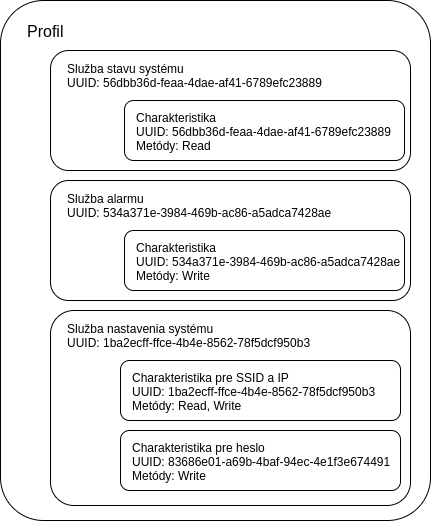
\includegraphics[scale=0.5]{obrazky-figures/BLE_structure.png}
    \caption{Štruktúra BLE služieb}
    \label{fig:BLE_structure}
\end{figure}

\section{Jednotka so senzorom}

Hlavnou časťou jednotky so senzorom je ESP32. Pre túto jednotku bola zvolená vývojová doska s~konektorom na batériu s~napätím až 3,7 voltov. ESP pomocou BLE komunikuje s~ústredňou. Konkrétny spôsob komunikácie je popísaný v~kapitole \ref{sec:komunikacia}. Okrem ESP je súčasťou jednotky aj samotný senzor a indikačná LED dióda. Tá sa rozsvieti v~prípade, že bolo zaznamenané narušenie priestoru. Táto jednotka musí podporovať minimálne PIR senzor a magnetický senzor. Všeobecne by však zariadenie malo podporovať akýkoľvek senzor, ktorý pri zistení narušenia dá na výstup napätie na úrovni logickej 1 prípadne 0. Táto časť nebola v~zadaní bližšie špecifikovaná, preto bola zvolená varianta, ktorou je možné zachytiť čo najväčšie spektrum senzorov.

\subsection{Použité senzory}

Medzi použité senzory boli zaradené najdostupnejšie senzory. Zároveň bol kladený dôraz aj na ich spotrebu. Senzory by pri tom mali byť schopné pri narušení oznámiť túto skutočnosť jednoduchým zmenením svojho výstupu na opačnú hodnotu.

\subsubsection{PIR senzor}

Pre PIR senzor bol vybraný senzor AM312, konkrétne modul zobrazený na obrázku \ref{fig:pir}. Je primárne navrhovaný na prácu pri izbových teplotách, s~napätím do 3,6 V~a prúdom do 100~$\mu$A. Dokáže pritom detekovať zmenu v~infračervenom poli až na vzdialenosť 3~-~5 metrov s~uhlom 100 až 130 stupňov v~závislosti na osi. Vďaka tomu je senzor použiteľný v~dvoch najbežnejších typoch - vejár a strop, viď rozdelenie typov PIR senzorov v~kapitole \ref{sec:pir}.\cite{pir-datasheet}
Tento senzor bol zvolený len v~prototype ako demonštrácia funkčnosti zariadenia, v~reálnom nasadení by mal byť použitý senzor s~nižším odberom energie. Existujú senzory so spotrebou len 1~-~6~$\mu$A v~pokojnom stave.\footnote{Napríklad senzory od spoločnosti Panasonic, špecifikácia dostupná na \url{https://b2b-api.panasonic.eu/file_stream/pids/fileversion/4541}}

\begin{figure}[ht]
    \centering
    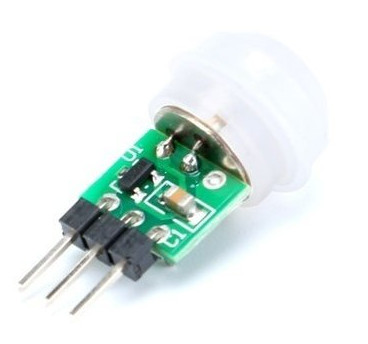
\includegraphics[scale=0.5]{obrazky-figures/pir.jpg}
    \caption[PIR senzor]{PIR senzor\footnotemark}
    \label{fig:pir}
\end{figure}
\footnotetext{prevzaté z: \url{https://www.laskarduino.cz/arduino-micro-pir-detektor-pohybu-am312}}

\begin{figure}[!ht]
    \centering
    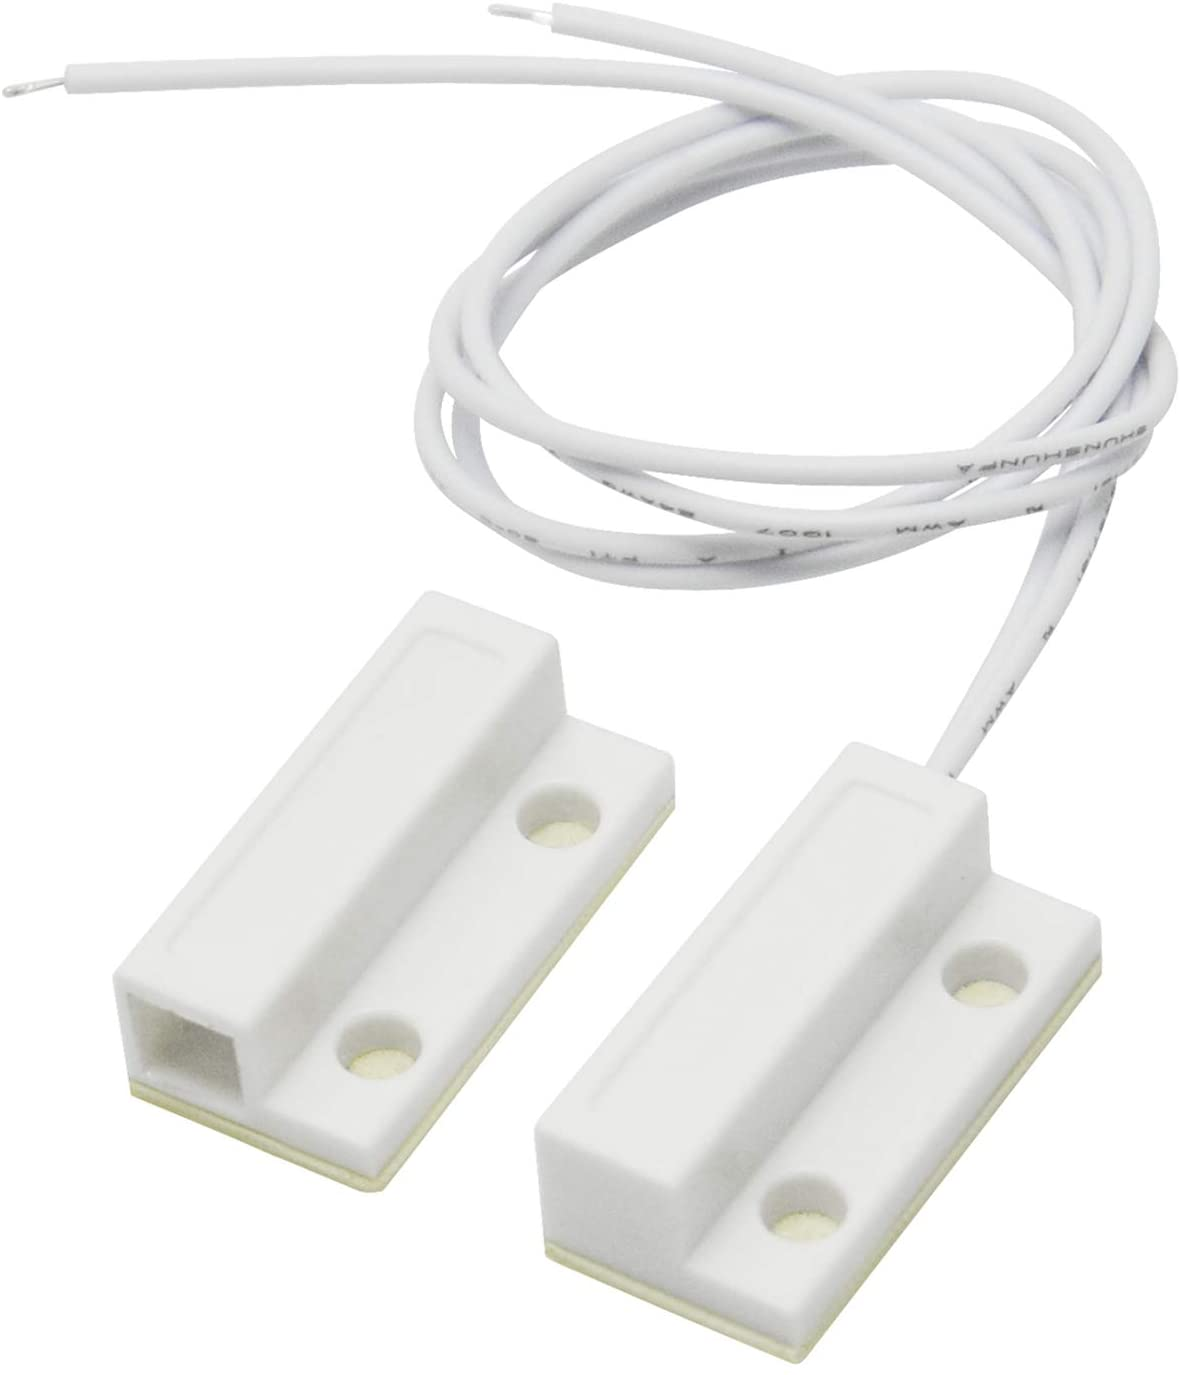
\includegraphics[scale=0.1]{obrazky-figures/magneticky_senzor.jpg}
    \caption[Magnetický senzor]{Magnetický senzor\footnotemark}
    \label{fig:magneticky_senzor}
\end{figure}
\footnotetext{prevzaté z: \url{https://www.amazon.co.uk/Gikfun-Sensor-Magnetic-Switch-Arduino/dp/B0154PTDFI}}

\subsubsection{Magnetický kontakt}

Pre magnetický senzor bol vybraný senzor MC-38, zobrazený na obrázku \ref{fig:magneticky_senzor}. Ten bol zvolený vďaka jeho dostupnosti, cene a jednoduchosti inštalácie. Jeho operačná vzdialenosť je 15 až 25 mm. Ide o~normálne uzavretý senzor, teda v~prítomnosti magnetu je jazýčkový kontakt zopnutý.


\subsection{Napájanie}

Napájanie jednotky so senzorom bude realizované pomocou batérie. Tým sa systém stane jednoduchším na inštaláciu a prípadne zmeny umiestnenia jednotlivých senzorov. Je však nutné, aby takéto napájanie vydržalo v~priemere aspoň rok. Pri výpočte vhodnej kapacity musíme počítať so spotrebou ESP32, ako aj so spotrebou samotného senzoru. Môžme pritom uvažovať niekoľko stavov:
\begin{itemize}
    \item systém je stále v~stave \textit{odstrážené}. Zariadenie je v~stave hlbokého spánku dlhšiu dobu.
    \item systém pravidelne strieda stavy. Ide o~očakávané zaobchádzanie so systémom. Počíta s~tým, že s~tým že systém je rovnaký čas v~oboch stavoch.
    \item systém je stále v~stave \textit{zabezpečené}. Ide o~extrém, kde je systém stále aktivovaný, teda hlboký spánok je obmedzený na kratšiu dobu. V~tomto prípade je spotreba energie najvyššia.
\end{itemize}

Týmto rozdelením môžme získať minimálnu, priemernú a maximálnu spotrebu systému. Podľa tabuľky \ref{tab:spotreba_esp} môžeme určiť, že spotreba modulu počas hlbokého spánku je 10~$\mu$A. Následne sa zariadenie prebudí a začne odosielať dáta pomocou BLE, je teda v~aktívnom stave. Keďže ide o~odosielanie dát počítame s~hornou hranicou 260~mA. Experimentami bolo zistené, že zariadenie ostane v~aktívnom stave maximálne po dobu 3,2 sekúnd. Odber zariadenia pri prebúdzaní pri tom zanedbáme nakoľko ide o~krátkodobú spotrebu a na výsledné meranie by nemala veľký vplyv.

Pri výpočte najprv zistíme koľko z~hodiny strávil senzor vo vybranom stave podľa nasledujúceho vzťahu:
$$(\text{počet cyklov za hodinu} * \text{čas strávený v stave}) / 3600$$

Tento čas vynásobíme spotrebou vo vybranom stave. Následne jednotlivé stavy spočítame a dostaneme spotrebu ESP32 za hodinu. K~tejto spotrebe je potrebné pripočítať spotrebu senzora. Túto celkovú spotrebu vynásobíme počtom hodín v~roku a dostaneme minimálnu kapacitu batérie potrebnú pre jednotku so senzorom.

V~nasledujúcom výpočte uvažujeme čas spánku 20 minút pri zabezpečenom systéme a 120 minút pri odstráženom stave. Kombinovanou hodnotou pri tom rozumieme spánok v~priemere 70 minút. Takto dostaneme nasledujúce hodnoty:

\begin{table}[ht]
    \centering
    \renewcommand{\arraystretch}{1.5}
    \begin{tabular}{|c|c|c|} \hline
        Stav systému                    & mód ESP          & spotreba za hodinu \\ \hline
        \multirow{2}{*}{zabezpečené}    & aktívny          & 691,489~$\mu$Ah \\ \cline{2-3}
                                        & hlboký spánok    & 9,973~$\mu$Ah \\ \hline
        \multirow{2}{*}{odstrážené}     & aktívny          & 115.504~$\mu$Ah \\ \cline{2-3}
                                        & hlboký spánok    & 9,996~$\mu$Ah \\ \hline
        \multirow{2}{*}{kombinované}    & aktívny          & 197,944~$\mu$Ah \\ \cline{2-3}
                                        & hlboký spánok    & 9,992~$\mu$Ah \\ \hline
    \end{tabular}
    \caption{Výpočet spotreby}
    \label{tab:spotreba_jednotky}
\end{table}

Celková kombinovaná spotreba systému je teda približne 207,936~$\mu$Ah, v~prípade, že započítame aj nami využitý senzor dostaneme sa na hodnotu 307,936~$\mu$Ah. Za rok tak systém spotrebuje 2697,519~mAh. V~prípade využitia úspornejšieho senzora by táto hodnota mohla byť podstatne nižšia. Ideálnym napájaním pre systém bude teda batéria s~kapacitou približne 2700~mAh a napätím 3,3~-~3,7~V. Tieto teoreticky zistené výpočty však nebolo možné potvrdiť meraním, preto predstavujú len odhad spotreby.

\section{Komunikácia ústredne so senzormi}\label{sec:komunikacia}

Pri komunikácií so senzormi sa využíva technológia BLE. Ústredňa vystupuje ako server, na ktorý sa pripájajú senzory ako klienti. Pri komunikácii sa využíva bonding, senzory sú teda trvalo spárované so základnou jednotkou a komunikácia prebieha v~šifrovanej podobe. V~kapitole \ref{sec:BLE_struc} je opísaná štruktúra serveru. Rozhodovanie senzoru je graficky znázornené na stavovom diagrame \ref{fig:sensor_state_diagram}. \textit{Stav} je hodnota prečítaná z~charakteristiky ústredne, \textit{alarm} je premenná uložená v~RTC pamäti mikrokontroléru, \textit{spánok} je čas, na ktorý je systém uvedený do hlbokého spánku.

\begin{figure}[ht]
    \centering
    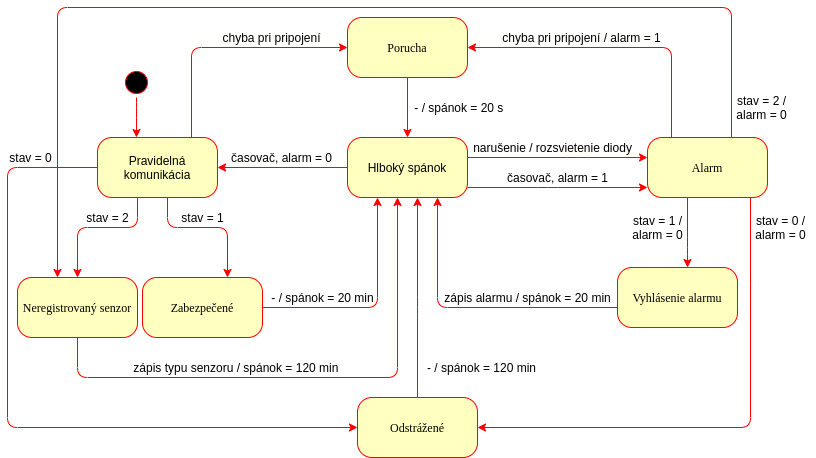
\includegraphics[width=\linewidth]{obrazky-figures/sensor_state_diagram.png}
    \caption[Stavový diagram senzoru]{Stavový diagram senzoru}
    \label{fig:sensor_state_diagram}
\end{figure}


Klient sa najprv pripojí na server a zistí stav ústredne prečítaním hodnoty služby. Následne podľa zisteného stavu urobí jedno z~nasledujúcich:
\begin{itemize}
    \item v~prípade, že senzor ešte nebol registrovaný, ústredňa odpovedá hodnotou 2. Informuje to tak senzor o~to, že ešte nebol konfigurovaný. Následne senzor odošle informáciu o~svojom type na ústredňu. Jeho registráciu je potrebné potvrdiť v~mobilnej aplikácii. Zároveň sa takýmto spôsobom zamedzuje zistenie stavu systému prípadnému narušiteľovi, ktorý by poznal spôsob komunikácie.
    \item ak je systém v~stave \textit{konfigurácie} alebo \textit{odstrážené} (ústredňa vrátila hodnotu 0), jednotka so senzorom sa uspí na 120 minút. Senzor je v~tomto prípade deaktivovaný. Tento spôsob je vhodný hlavne pre šetrenie batérie jednotky.
    \item v~ostatných stavoch sa jednotka so senzorom uspí na 20 minút. Zároveň sa aktivuje prebudenie jednotky pomocou senzora. V~prípade prebudenia zo senzora sa na príslušnú službu serveru zapíše oznámenie o~narušení.
\end{itemize}

Po všetkých variantách sa jednotka so senzorom uspí na stanovený čas. Pri uspávaní sa využije mód hlbokého spánku, ktorý patrí medzi najúspornejšie pričom dokáže stále prebudiť systém z~externého zdroja. Týmto externým zdrojom je v~tomto prípade čidlo, ktoré pri zaznamenaní narušenia automaticky jednotu prebudí. Po prebudení senzor znova oznámi svoju funkčnosť ústredni a zistí stav systému. Rozhodovanie sa opakuje.

Jednotlivé rozostupy medzi overeniami dostupnosti senzorov boli zvolené na základe tabuľky \ref{tab:interval_overenia}. Je dôležité zvoliť správne rozostupy pre zabezpečenie čo najčastejšej komunikácie a zároveň udržanie čo najnižšej spotreby jednotiek so senzormi. Spomínané rozostupy platia len pre pravidelnú komunikáciu, ktorou sa overuje dostupnosť senzorov. V~prípade, že senzor zaznamená narušenie, jednotka je okamžite prebudená.

V~prípade, že sa senzoru nepodarí kontaktovať ústredňu uspí sa na 20 sekúnd, po ktorých toto odosielanie znova opakuje. Ústredňa pravidelne kontroluje dostupnosť senzorov. Ak sa senzor neohlási po očakávanej dobe podľa aktuálneho stavu, dostane ďalšie 2 možnosti na nadviazanie komunikácie. V~prípade že sa ani po tejto dobe nepodarí senzoru pripojiť, je vyhlásený za nedostupný a systém je prepnutý do stavu poruchy, respektíve je vyvolaný poplach kvôli sabotáži senzoru.

\section{Správa systému}

Celý systém je potrebné spravovať. Keďže samotný systém neobsahuje žiadnu zobrazovaciu jednotku, ako je displej, nie je možné túto správu vykonávať priamo z~ústredne. Túto funkciu v~navrhovanom systéme bude zastrešovať mobilná aplikácia. Tá by sa mala postarať o~nasledovné funkcie:
\begin{itemize}
    \item \textbf{počiatočné nastavenie systému} - slúži na nastavenie názvu a hesla Wi-Fi siete, na ktorú sa má zariadenie pripojiť. Následne sa odošle odpoveď z~ústredne v~podobe IP adresy ústredne.
    \item \textbf{zmena číselného kódu} - zmena aktuálneho kódu, ktorý slúži na deaktiváciu systému a prepnutie do stavu konfigurácie.
    \item \textbf{správa senzorov} - zobrazenie základných informácií o~senzore, pridávanie nových senzorov, prípadne ich odoberanie.
    \item \textbf{správa spárovaných zariadení} - pridávanie nových zariadení, odstraňovanie zariadení. Slúžia na automatickú deaktiváciu systému. Zároveň by aplikácia mala podporovať nastavenie vzdialenosti, na ktorú bude ústredňa tieto zariadenia registrovať.
    \item \textbf{aktivácia systému} - aktivácia systému pomocou aplikácie, teda prepnutie do stavu aktivácie a následne do stavu zabezpečené.
\end{itemize}

Odosielanie takmer všetkých požiadaviek na ústredňu bude prebiehať pomocou HTTP požiadaviek na lokálnej sieti. Je teda nutné, aby obe zariadenia boli pripojené na rovnakú Wi-Fi sieť. Výnimkou budú počiatočné nastavenia, ktoré slúžia práve na nastavenie komunikácie pomocou Wi-Fi. Tieto počiatočné nastavenia budú prebiehať pomocou technológie BLE. Pri všetkých nastaveniach musí byť systém v~stave konfigurácie. Jedinou výnimkou je aktivácia systému, ktorá okrem stavu konfigurácie podporuje aj stav odstrážené.

Využitie HTTP oproti BLE ponúka jednoduchšiu komunikáciu, nevyžaduje od užívateľa zapnutie dvoch technológií - služby polohy a Bluetooth. Služby polohy sú pre novšie operačné systémy nutné pre skenovanie okolitých Bluetooth zariadení. Zároveň využitie HTTP môže byť v~budúcnosti rozšírené pre komunikácie aj mimo lokálnu sieť, napríklad zaslanie notifikácie o~alarme a podobne. 

Pre čo najväčšiu kompatibilitu medzi platformami je najvhodnejšie využiť štandardné webové technológie ako sú HTML, CSS a Javascript. Pre jednoduchší prístup k~zariadeniu a zároveň ušetrenie pamäti na ESP bola zvolená varianta s~hybridnou aplikáciou. Vďaka tomu funguje ESP len ako aplikačný server a nie je nutné na ňom uchovávať ďalšie informácie v~pomerne malej pamäti. Očakáva sa, že aplikácia bude pravidelne používaná na kontrolu systému, prípadne občasné zmeny v~nastaveniach zabezpečovacieho systému. Konkrétne bol pre aplikáciu zvolený Framework7, ktorý je postavený na Apache Cordova. Ide o~pravidelné aktualizovaný a stále vyvíjaný nástroj. Do aplikácie je pri tom stále možné pridávať ďalšie moduly vyvinuté pre Apache Cordoba.

\chapter{Implementácia}

Samotná implementácia prototypu sa skladá z~dvoch na seba nadväzujúcich častí. Prvou sú programy pre vstavaný systém, teda pre mikrokontrolér ESP32. Ide o~program pre ústredňu a program pre jednotku so senzorom. Druhou časťou je mobilná aplikácia pre správu systému a zobrazenie aktuálnych informácií o~zabezpečovacom systéme. V~kapitole je následne popísaná aj konkrétna komunikácia medzi zariadeniami v~systéme.

\section{ESP32}

Z~dostupných možností pre implementáciu bol vybraný framework ESP IDF ako najvhodnejší. Ten sa ukázal ako najlepší pre komunikáciu pomocou BLE, komunikácia je pomerne jednoduchá s~veľkou mierou konfigurácie. Framework poskytuje zároveň veľké množstvo príkladov, ktoré demonštrujú jednotlivé funkcie a možnosti použitia. Dostupná je tiež pomerne obsiahla dokumentácia\footnote{Dostupná z: \url{https://docs.espressif.com/projects/esp-idf/en/latest/esp32/}}, ktorá pomôže najmä s~inštaláciou a nastavením systému. Zároveň obsahuje aj popis jednotlivých funkcií a ich parametrov. Tá bola spolu s~príkladmi zároveň využitá na oboznámenie sa so spôsobom programovania jednotlivých súčastí systému. Niektoré časti kódu boli s~malými úpravami priamo prevzaté z~týchto príkladov. Išlo napríklad o~základnú kostru komunikácie pomocou Wi-Fi a Bluetooth Low Energy.

\subsection{Ústredňa}

Ústredňa systému sa stará o~niekoľko rôznych činnosti, tie sú samostatne rozdelené na úlohy (task). To umožňuje systému pravidelne opakovať činnosti ako je čítanie hodnôt z~klávesnice, indikácia alarmu a podobne. Pri spustení ústredne sa najprv načíta konfigurácia systému uložená v~stálej pamäti (non-volatile memory). Tá obsahuje kód pre odstráženie systému, počet senzorov, adresy jednotlivých senzorov, meno a heslo Wi-Fi siete. Okrem týchto informácii systém automaticky ukladá aj adresy spárovaných zariadení a k~nim patriace kľúče. Po načítaní celej konfigurácie nasleduje prípadné pripojenie k~Wi-Fi sieti, inicializácia aplikačného rozhrania systému, synchronizácia aktuálneho času pomocou protokolu SNTP (Simple Network Time Protocol) a inicializácia jednotlivých štruktúr potrebných pre komunikáciu pomocou BLE. 

Samotný program pre ústredňu sa skladá z~niekoľkých častí rozdelených do logických celkov podľa funkcie. Jednou z~hlavných častí je komunikácia pomocou BLE. Ústredňa sa pri tom správa ako server pri komunikácii so senzormi, ale zároveň ako klient pri komunikácii so známymi zariadeniami. Väčšina BLE nositeľných zariadení totiž funguje ako server pre zníženie spotreby energie. Pri oboch typoch komunikácie ústredňa stále nadväzuje šifrované spojenie. Po aktivácii systému ústredňa pravidelne skenuje okolie pre dostupné zariadenia. Najprv prebieha selekcia na základe vzdialenosti od ústredne pomocou hodnoty sily signálu~--~RSSI (received signal strength indicator). Následne prebieha hľadanie známych zariadení. Ak sa takéto zariadenie nájde, ústredňa sa pokúsi k~nemu pripojiť. V~prípade úspešného pripojenia následne mení svoj stav na deaktivované.

Hodnota RSSI je nastaviteľná z~mobilnej aplikácie. Užívateľ v~aplikácii zadá desatinným číslom maximálny počet metrov, na ktorý má systém zaznamenávať zariadenia. Táto hodnota je zaslaná na ústredňu kde je prepočítaná na hodnotu RSSI a následne uložená v~pamäti. Prepočet prebieha pomocou vzorca:

$$\text{RSSI} = \text{faktor prostredia} * (- 10) * \log_{10}(\text{vzdialenosť}) + \text{RSSI jedného metra}$$

\textit{Faktor prostredia} označuje konštantu podľa prostredia. V~našom prípade je prostredie vo vnútri domu alebo bytu, kde je pomerne dosť prekážok, preto je táto konštanta zvolená na maximum~--~4. \textit{RSSI jedného metra} je hodnota RSSI na vzdialenosť jedného metra. Táto hodnota je vypočítaná z~vysielacieho výkonu zariadenia. V~systéme sa táto hodnota nemení, na začiatku inicializácie ústredne sa nastaví na maximálnu podporovanú úroveň +9~dbm. Ide o~približný výpočet a výsledná hodnota sa mení v~závislosti na umiestnení zariadení a podobne. Vzorec je možné označiť ako tradičný výpočet RSSI zo vzdialenosti.\footnote{Dostupné napríklad z: \url{https://forums.estimote.com/t/determine-accurate-distance-of-signal/2858/5}}

Ústredňa očakáva v~pravidelných intervaloch pripojenie senzora. Ak toto spojenie nie je opakovane nadviazané, systém túto skutočnosť indikuje rozsvietením diódy, ktorá okrem poruchy oznamuje, že systém nie je možné prepnúť do stavu stráženia. V~prípade pokusu o~aktiváciu systému je užívateľ upozornený ako vizuálne tak aj akusticky. Senzor je zaznamenaný pri pripojení a následnom prečítaní charakteristiky definujúcej stav systému. Zaznamená sa čas v~podobe časovej známky a vynuluje sa počítadlo označujúce koľkokrát sa jednotka neozvala. Ďalej môže nasledovať zápis do služby alarmu, ten je zaznamenaný, uchovávajú sa pri tom informácie o~tom, ktorý senzor a kedy tento alarm spustil. Následne sú spustené indikácie alarmu.

Pre záložný spôsob deaktivácie alarmu a základnú interakciu priamo s~ústredňou bola zvolená maticová číselná klávesnica o~veľkosti 4x3. Využíva sa známy princíp striedania výstupu po stĺpcoch a načítavanie hodnôt po riadkoch. Pri opakovanom zadaní nesprávneho kódu na deaktiváciu systému je spustený alarm. Toto počítadlo je vynulované pri zadaní správneho kódu. Maximálna podporovaná dĺžka kódu je 18 znakov. Pri presiahnutí tohto rozsahu sa kód vyčistí a nový znak je pridaný do prázdneho kódu.

Ústredňa implementuje aj vlastné aplikačné rozhranie, pomocou ktorého sú odosielané a prijímané požiadavky z~aplikácie. V~prípade, že systém nie je v~stave konfigurácie, ústredňa odpovie chybovým kódom a nevykoná sa žiadna zmena. Samotný obsah požiadaviek a odpovedí je odosielaný vo formáte JSON.


\subsection{Jednotka so senzorom}

Hlavnou časťou programu pre senzor je komunikácia pomocou Bluetooth Low Energy. Jednotka po prebudení inicializuje štruktúry potrebné pre samotnú komunikáciu. Nasleduje vyhľadávanie hlavnej jednotky. Senzor sa snaží o~pripojenie k~ústredni a zistenie jej stavu. V~prípade, že sa pripojenie nepodarilo, jednotka sa uspí na niekoľko sekúnd a pokúsi sa znova pripojiť. Ak bolo zároveň zaznamenané narušenie, jednotka si túto informáciu uloží do RTC pamäte. Ako bolo opísané v~kapitole \ref{sec:esp-sleep}, táto pamäť nie je zmazaná ani počas hlbokého spánku. Pri ďalšom prebudení sa pokúsi znova toto narušenie nahlásiť.

V~prípade úspešného pripojenia, jednotka prečíta aktuálny stav systému. Ak bola jednotka prebudená narušením zo senzora a systém je v~stave \textit{zabezpečené}, zapíše túto informáciu do príslušnej BLE charakteristiky. Pri tejto komunikácií sa vymieňajú číselné hodnoty, ktoré reprezentujú jednotlivé stavy. V~prípade, že išlo o~prebudenie časovačom, jednotka ohlási svoju prítomnosť ústredni spárovaním a prečítaním BLE charakteristiky. Podľa stavu systému sa nastaví čas, po ktorom bude jednotka znova prebudená.

Program pre jednotku so senzorom je zdieľaný pre oba typy senzorov. Pri programovaní mikrokontroléru je potrebné v~konfigurácii vybrať typ senzoru. Tým sa zmení spôsob prebudenia mikrokontroléru. Podľa tohto nastavenia zároveň senzor oznamuje svoj typ ústredni pri prvom pripojení. Konfiguráciu je možné meniť pomocou príkazu \textit{idf.py menuconfig}. Samotné nastavenie je v~kategórii s~názvom \textit{Sensor configuration}.

V~prototype je senzor napájaný jednou batériou typu 18650 s~kapacitou 2600 mAh, čo by podľa teoretických výpočtov malo vystačiť na takmer rok prevádzky jednotky so senzorom bez potreby výmeny batérie.

\section{Mobilná aplikácia}

Pre implementáciu aplikácie bol využitý Framework7 vo verzi 5.5 a React. Na programovanie bol teda z~väčšej časti využitý jazyk Typescript. Aplikácia pre komunikáciu pomocou BLE aplikácia využíva prídavný modul \textit{bluetoothle}\footnote{Dostupný z: \url{https://github.com/randdusing/cordova-plugin-bluetoothle}}. Podporuje pri tom Android od verzie 6.0, Windows 10 a iOS od verzie 8. Tento modul je využívaný na skenovanie okolitých zariadení. Hľadá sa pri tom zariadenie podľa názvu, unikátneho identifikačného čísla služby a charakteristiky. Následne sa využíva aj na samotné pripojenie, zápis a prečítanie údajov z~charakteristiky.

Samotná aplikácia je rozdelená na niekoľko obrazoviek podľa ich funkcie. Na hlavnej obrazovke sú zobrazené základne informácie o~systéme spolu s~tlačidlom pre aktiváciu systému. V~dolnej časti stránky sa nachádza aj navigácia na ďalšie stránky, prípadne tá je dostupná aj v~ľavom menu aplikácie. 

\begin{figure}[!ht]
    \centering
    \begin{subfigure}{.4\textwidth}
      \centering
      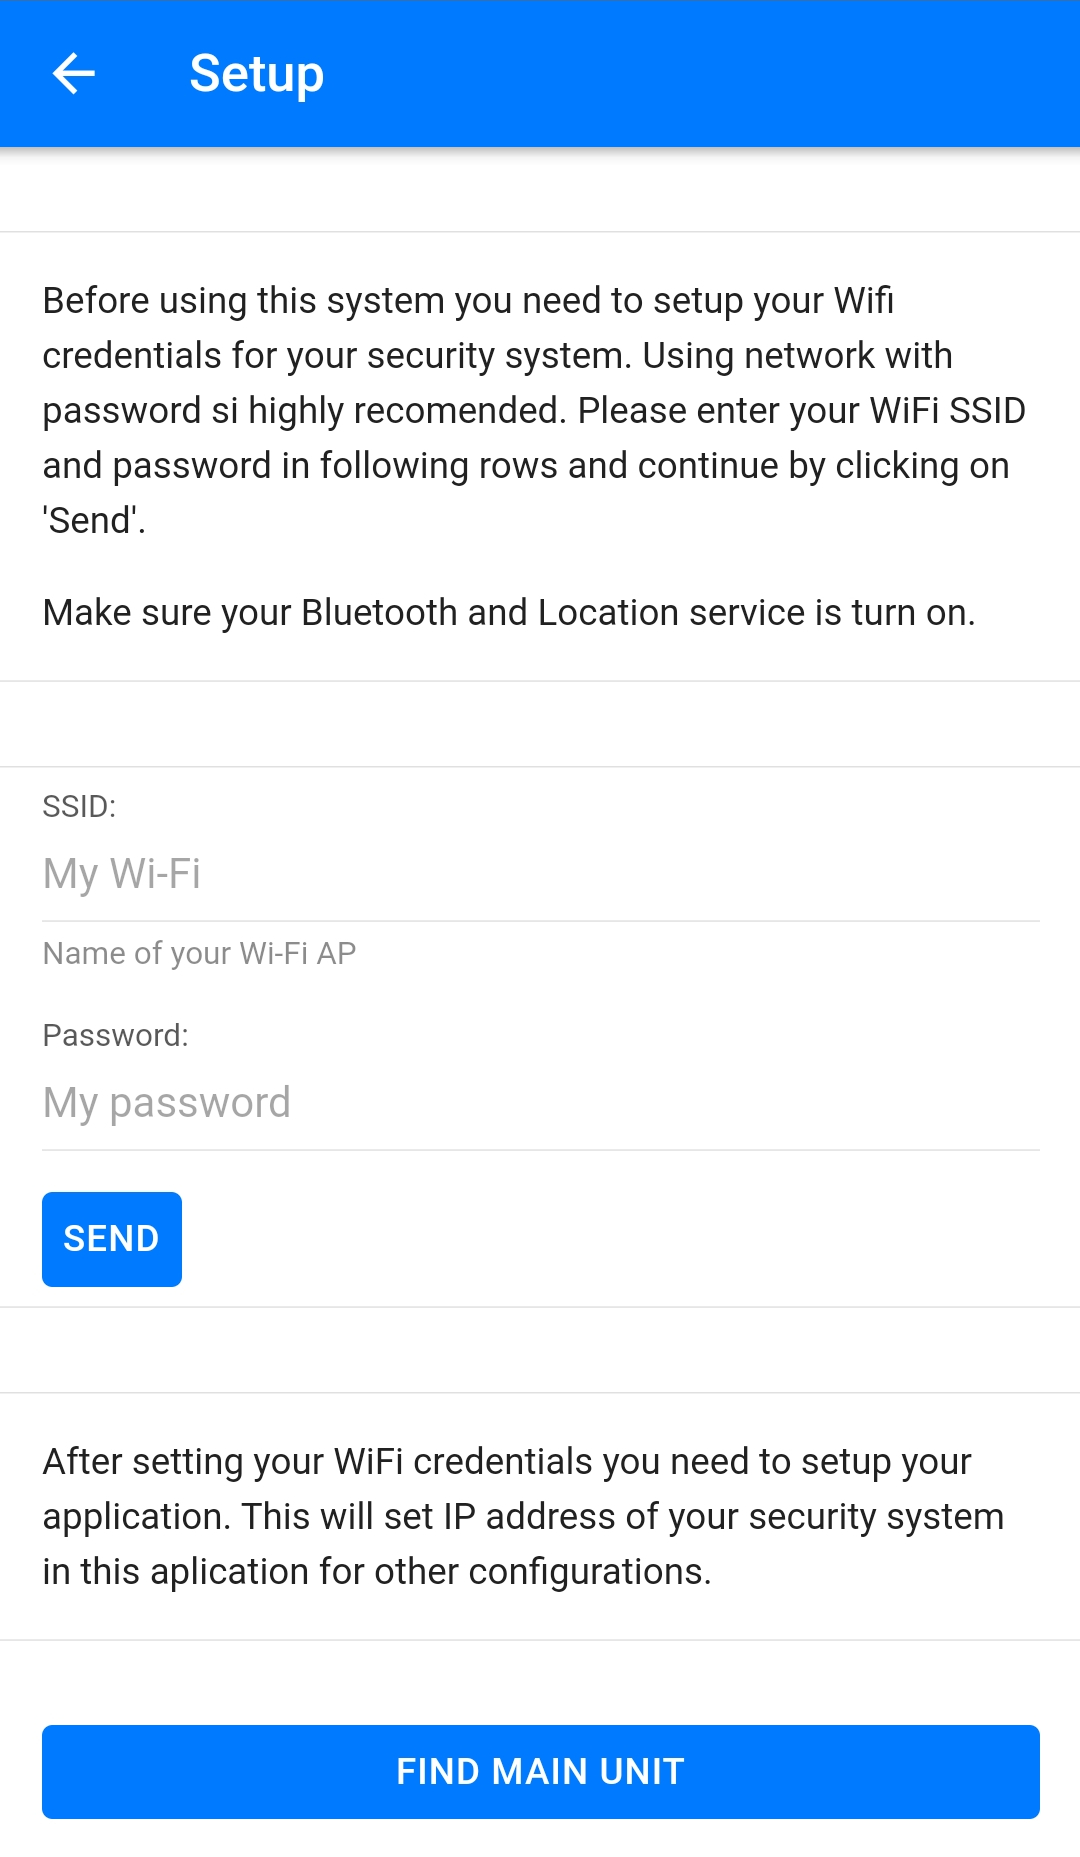
\includegraphics[width=.8\linewidth]{obrazky-figures/screen_setup.jpg}  
      \caption{Setup}
      \label{fig:screen_setup}
    \end{subfigure}
    \begin{subfigure}{.4\textwidth}
      \centering
      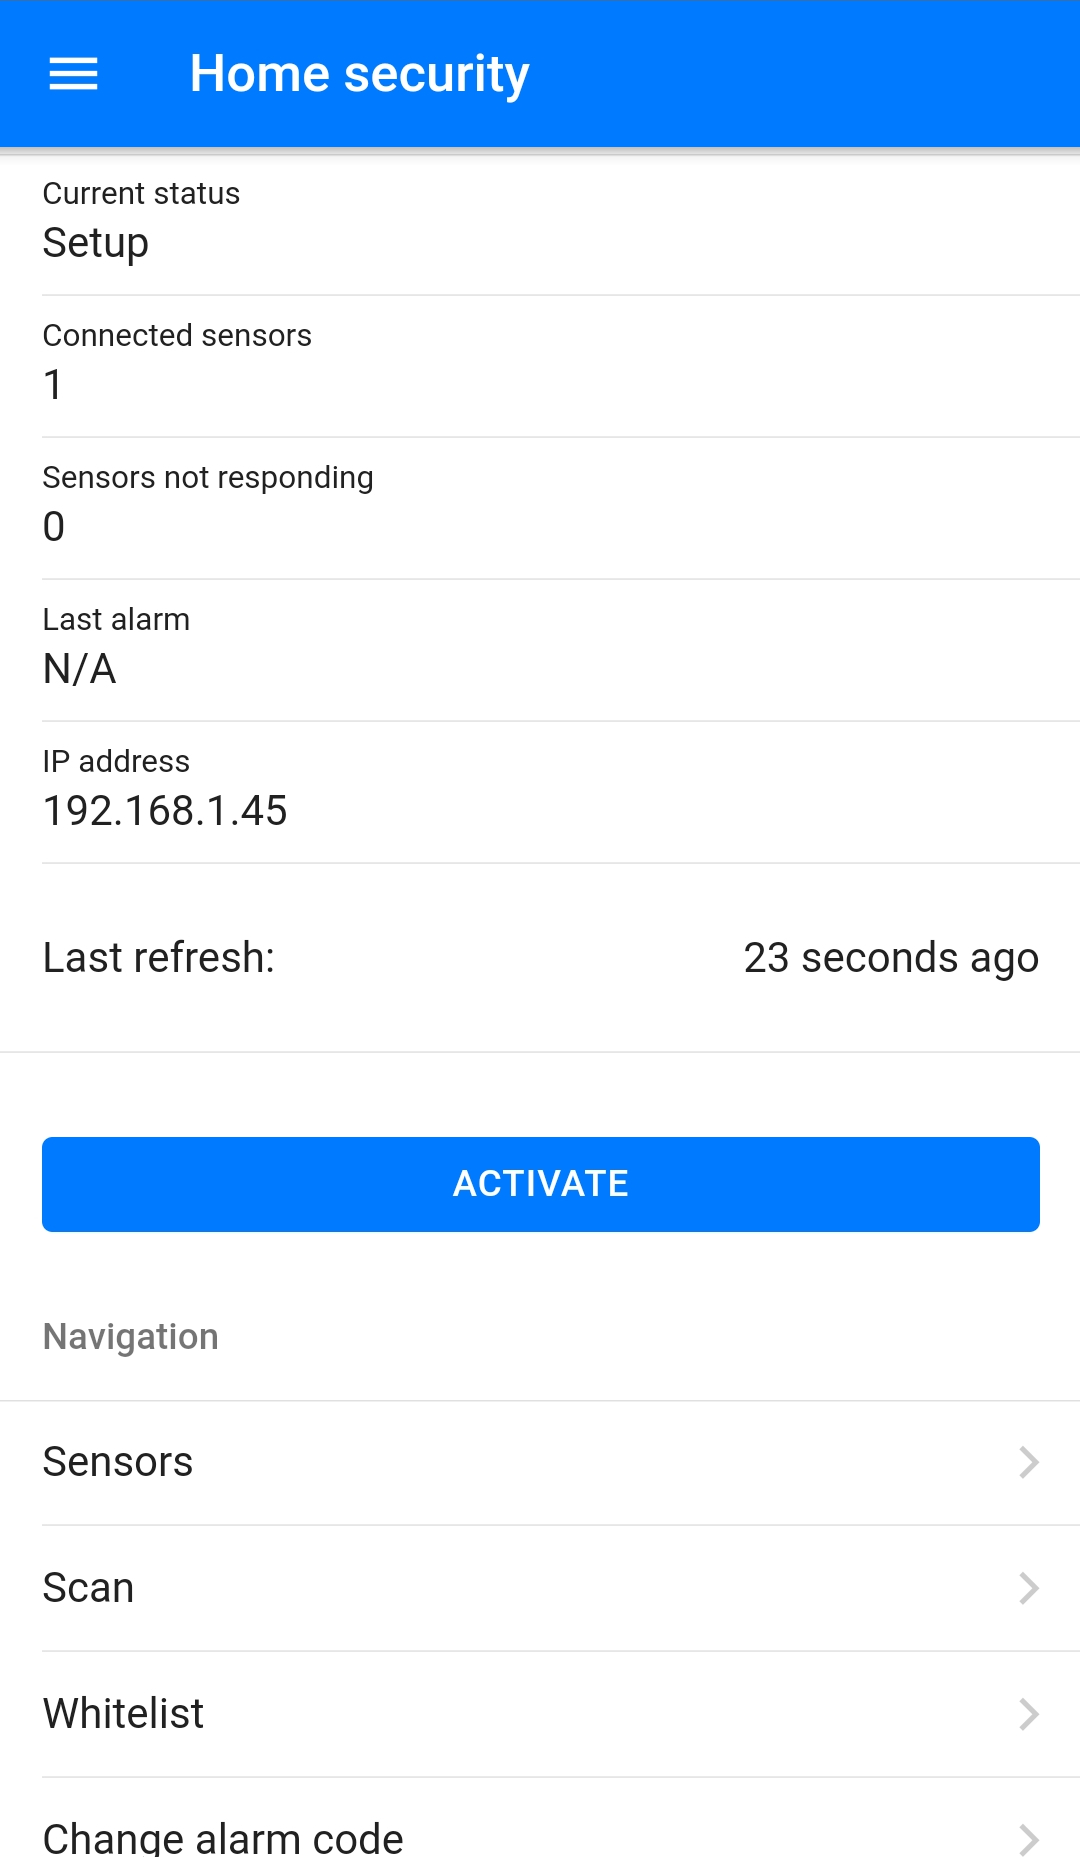
\includegraphics[width=.8\linewidth]{obrazky-figures/screen_home.jpg}  
      \caption{Home}
      \label{fig:screen_home}
    \end{subfigure}
    \caption{Nastavenie aplikácie}
    \label{fig:nastavenie_aplikacie}
\end{figure}

Pri prvom spustení mobilnej aplikácie je užívateľ presunutý na obrazovku s~nastavením aplikácie, kde je potrebné vyplniť názov a heslo Wi-Fi siete. Toto nastavenie je dostupné len ak je ústredňa v~stave \textit{konfigurácie}. Pri prvom spustení je ústredňa automatický do tohto stavu prepnutá. Následne pri nastavení ďalšej aplikácie je však nutné znova prepnúť ústredňu do tohto stavu. Zamedzuje sa tak nepovolenému prístupu k~systému. Snímok obrazovky z~tohto nastavenia je zobrazený na obrázku \ref{fig:screen_setup}. Pri úspešnom odoslaní údajov je nutné počkať na reštart systému. Skončenie nastavovania je oznámené krátkym pípnutím, po ktorom je ešte nutné získať IP adresu ústredne pre následnú komunikáciu pomocou HTTP. Po získaní adresy je užívateľ automaticky presunutý na domovskú stránku aplikácie odkiaľ sa môže prepnúť na ďalšie nastavenia. V~hornej časti obrazovky sú zobrazené aktuálne informácie o~systéme. Tie sú automaticky aktualizované v~intervale 30 sekúnd. V~prípade neúspešnej aktualizácie údajov je užívateľ informovaný o~nedostupnosti ústredne. V~spodnej časti stránky sa nachádzajú skratky pre rýchlu navigáciu medzi obrazovkami aplikácie. Tá je tiež prítomná v~menu aplikácie dostupnom v~ľavom hornom rohu obrazovky. Ukážku domovskej obrazovky je možné vidieť na obrázku \ref{fig:screen_home}.

\begin{figure}[!ht]
    \centering
    \begin{subfigure}{.4\textwidth}
      \centering
      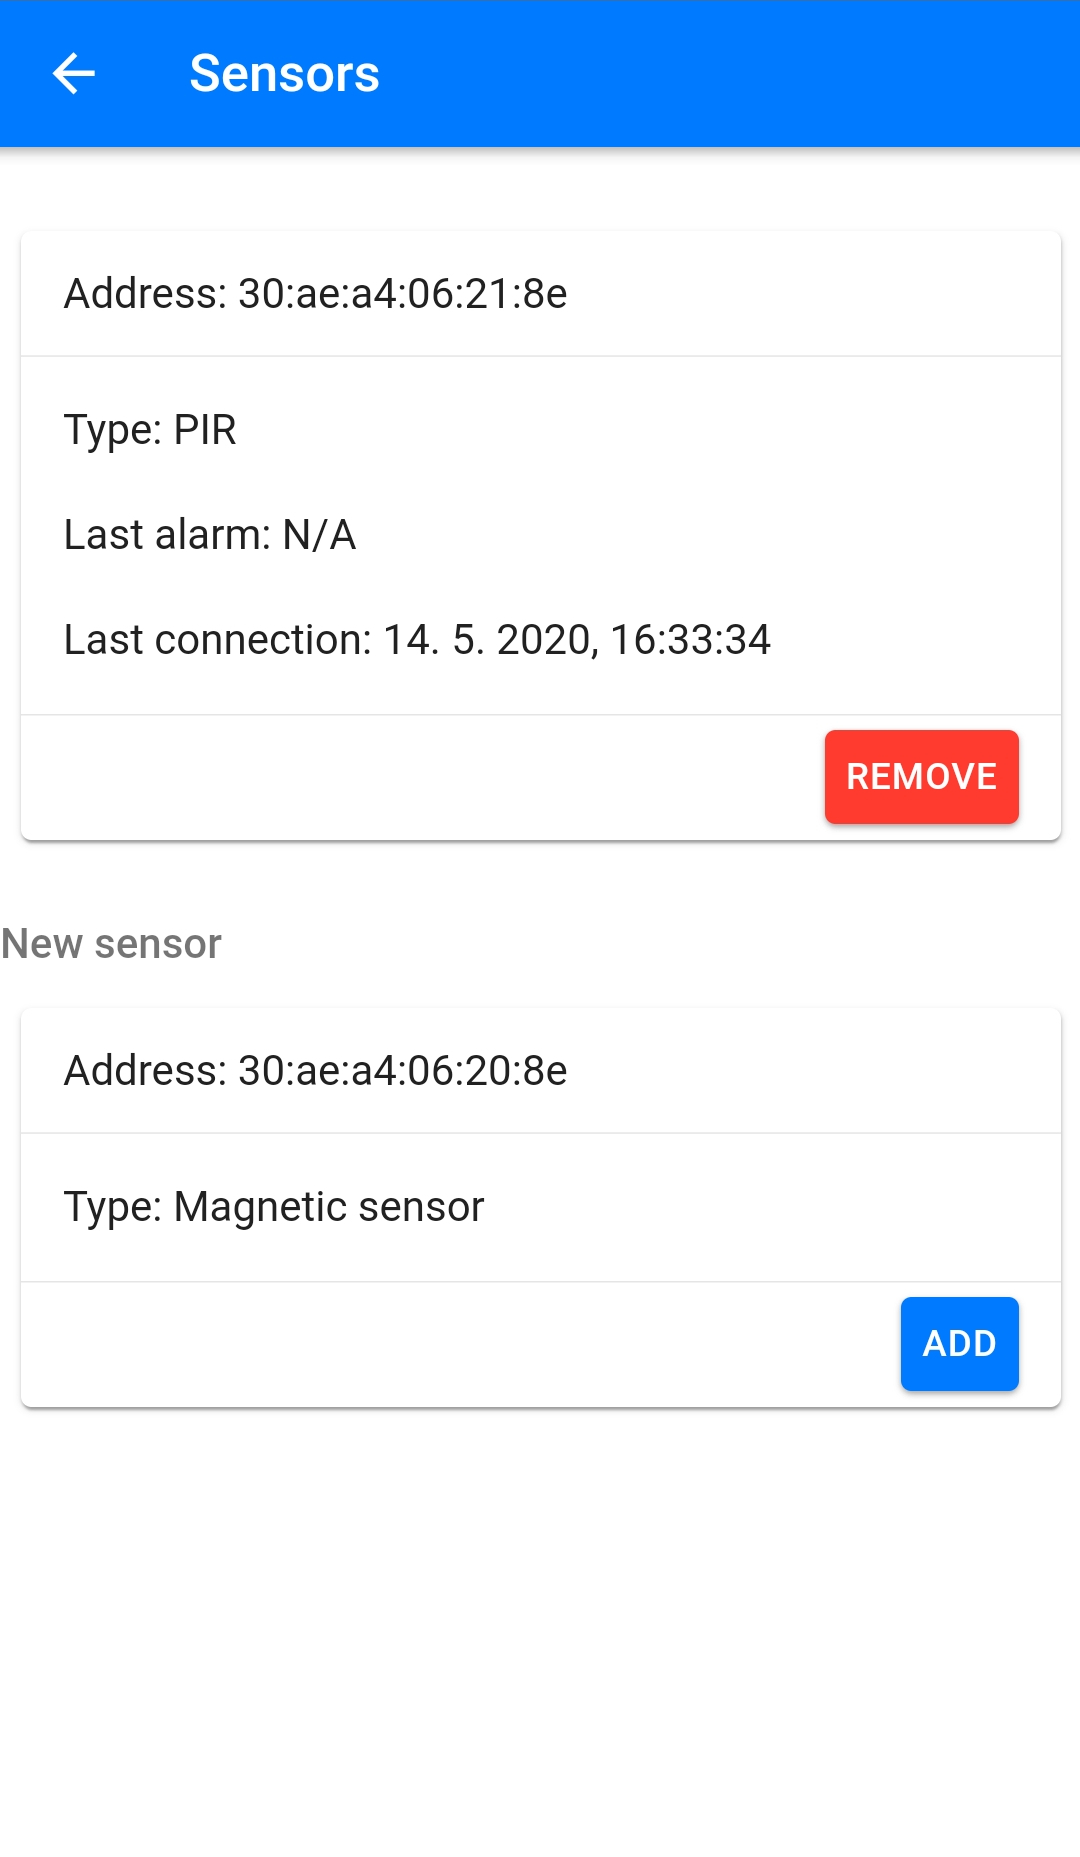
\includegraphics[width=.8\linewidth]{obrazky-figures/screen_sensors.jpg}
      \caption{Senzory}
      \label{fig:screen_sensors}
    \end{subfigure}
    \begin{subfigure}{.4\textwidth}
      \centering
      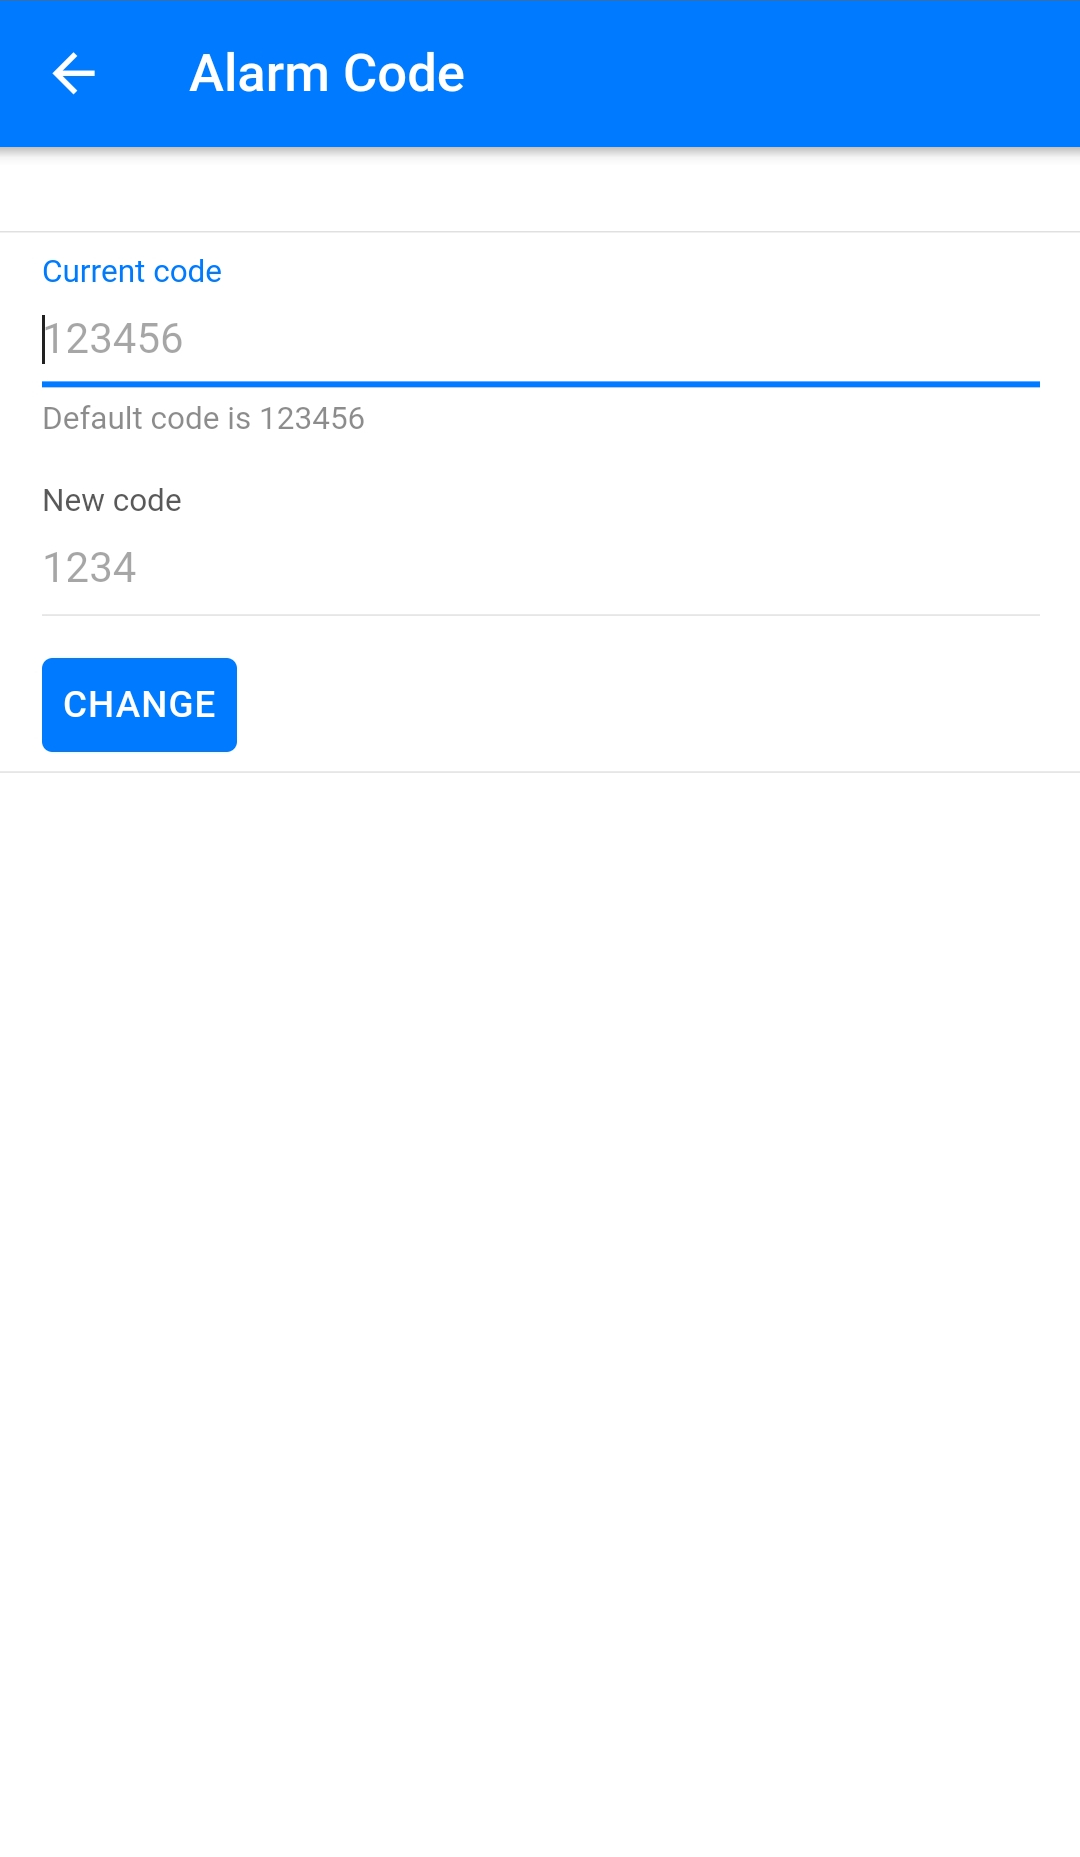
\includegraphics[width=.8\linewidth]{obrazky-figures/screen_code.jpg}  
      \caption{Zmena kódu zabezpečenia}
      \label{fig:screen_code}
    \end{subfigure}
    \caption{Nastavenia zabezpečenia}
    \label{fig:nastavenie_zabezpecenia}
\end{figure}

Následne je potrebné definovať jednotlivé senzory systému. Tie sa pri prvom pripojení registrujú do aplikácie. Registrácia prebieha po jednom senzore. V~aplikácii je možné vidieť aktuálne senzory plus prípadne jeden nový, ktorý naposledy žiadal o~spárovanie. Pre registráciu nového senzoru musí byť systém v~stave konfigurácie. Príklad s~jedným registrovaným a jedným novým senzorom je zobrazený na obrázku \ref{fig:screen_sensors}. Tu je možné vidieť typ senzora, pri už registrovaných senzoroch aj ich poslednú komunikáciu a naposledy spustený alarm. Následne sa odporúča zmena číselného kódu, ktorým sa systém deaktivuje, jeho nastavenie je zobrazené na obrázku \ref{fig:screen_code}. Aplikácia obsahuje aj nápovedu pre prvotný kód.

\begin{figure}[!ht]
    \centering
    \begin{subfigure}{.4\textwidth}
      \centering
      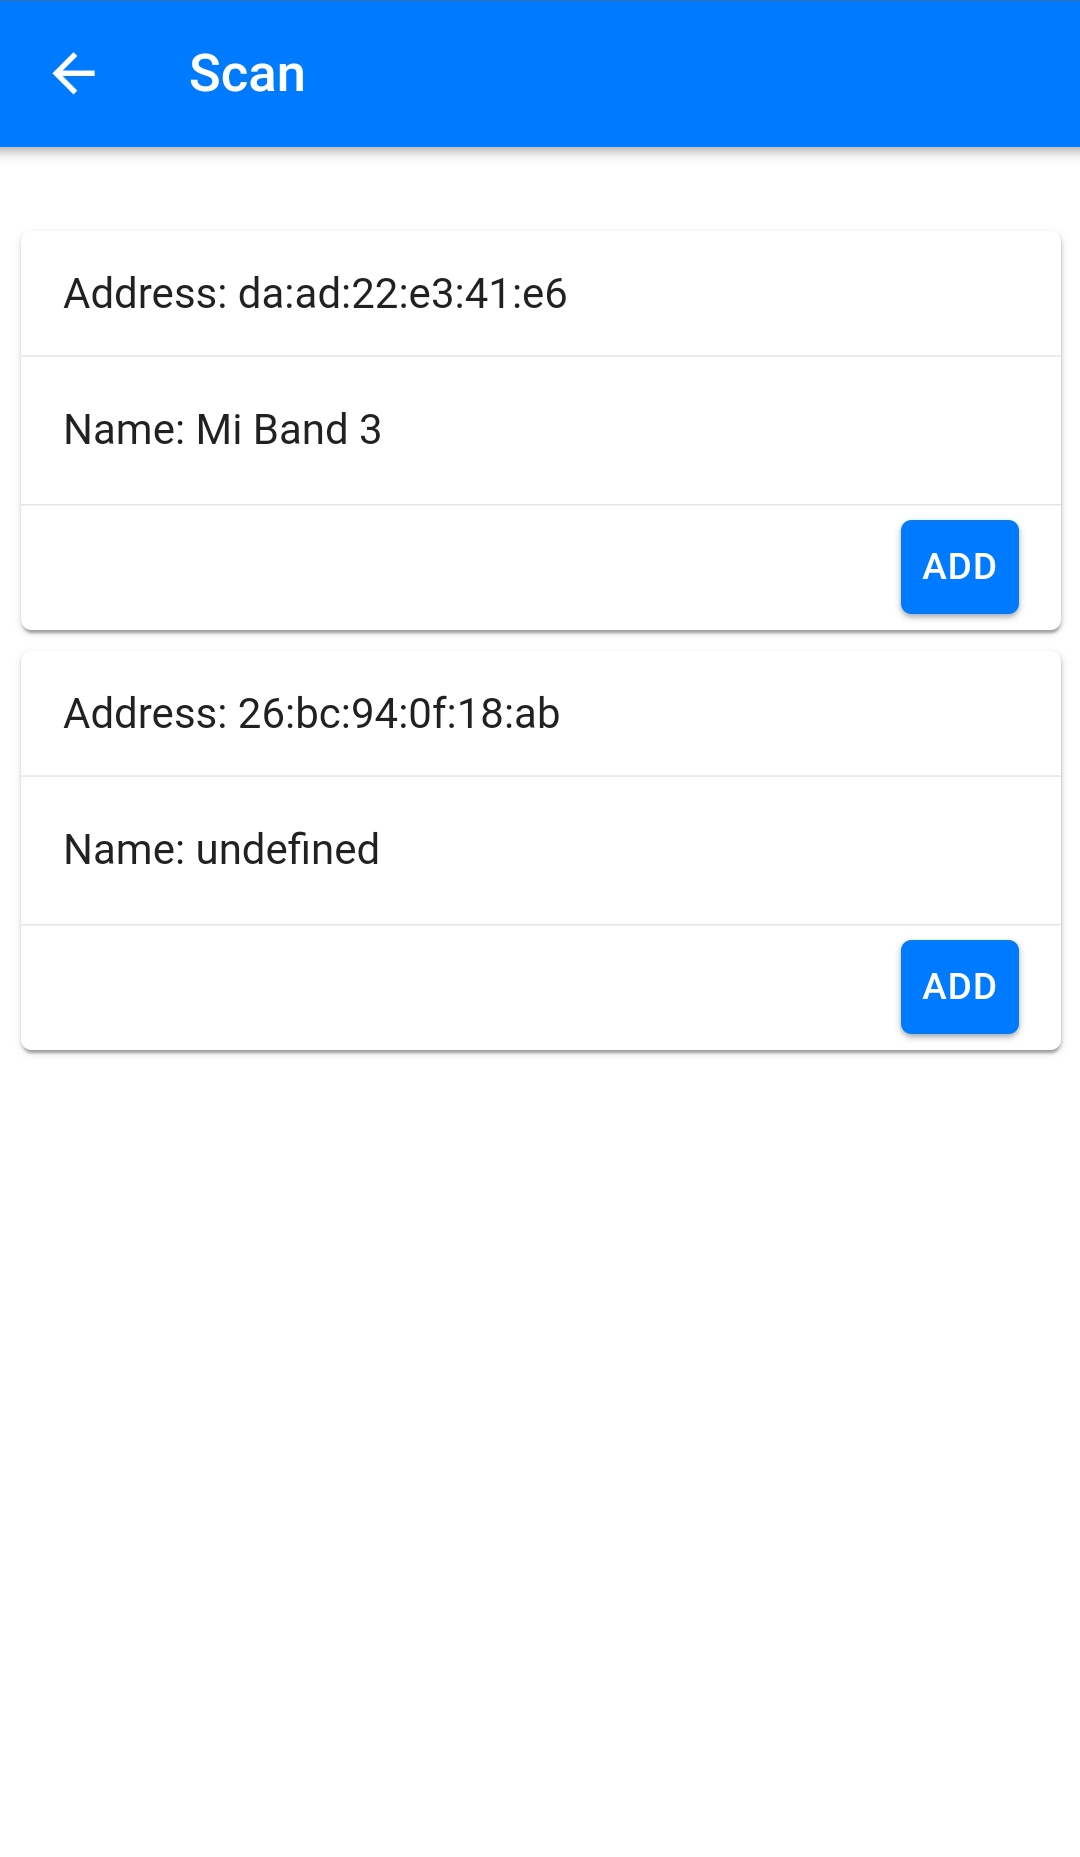
\includegraphics[width=.8\linewidth]{obrazky-figures/screen_scan.jpg}
      \caption{Vyhľadávanie nových zariadení}
      \label{fig:screen_scan}
    \end{subfigure}
    \begin{subfigure}{.4\textwidth}
      \centering
      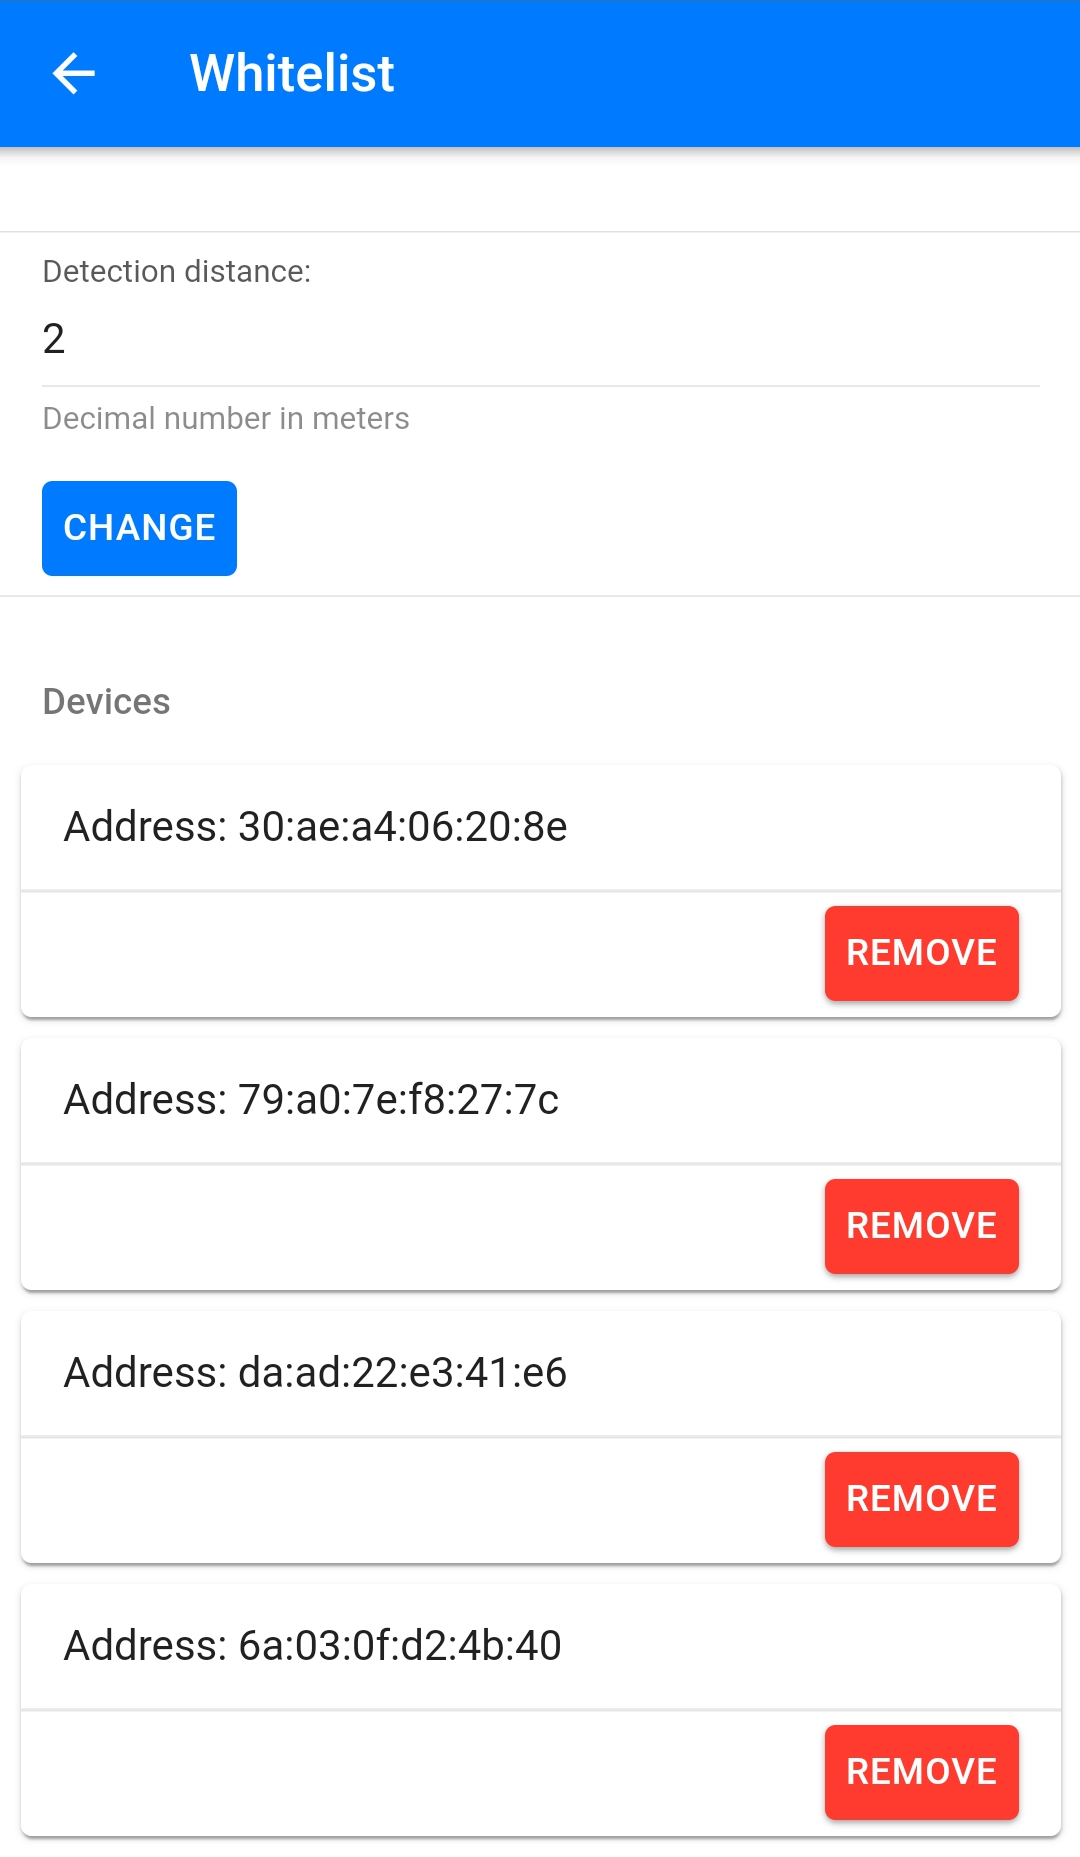
\includegraphics[width=.8\linewidth]{obrazky-figures/screen_whitelist.jpg}
      \caption{Definované zariadenia}
      \label{fig:screen_whitelist}
    \end{subfigure}
    \caption{Nastavenia detekcie zariadení}
    \label{fig:nastavenie_ble_zariadeni}
\end{figure}

Ďalším krokom by malo byť definovanie BLE zariadení, ktoré automaticky deaktivujú systém. Pri pridávaní nových zariadení prebieha sken pre okolité zariadenia. Príklad výsledku skenovania zariadení je zobrazený na obrázku \ref{fig:screen_scan}. Zariadenia, ktoré sú spárované so systémom je následne možné prehliadať a vymazávať na stránke zobrazenej na obrázku \ref{fig:screen_whitelist}. Na tejto stránke je zároveň možné zmeniť vzdialenosť, na ktorú sú zariadenia detekované.


\section{Testovanie}

Systém bol testovaný vo vnútri v~domácom prostredí pre simulovanie podmienok, do ktorých je primárne navrhovaný. Pre účely testovania systému bolo nutné upraviť rozostupy medzi komunikáciou ústredne so senzormi. Tie boli podstatne skrátené na niekoľko desiatok sekúnd, aby bolo možné sledovať správanie systému v~prípade výpadku senzora. Nedostupnosť senzora bola testovaná priamo odpojením jeho napájania a následného sledovania reakcie ústredne. Test prebehol úspešne a ústredňa dokázala zistiť chýbajúci senzor a zároveň v~aplikácii oznámiť túto skutočnosť. Pri opätovnom zapojení senzora sa ústredňa dokázala vrátiť do pôvodného stavu. Dosah ústredne na senzory sa pri testovaní ukázal ako priemerný, ale stále postačujúci na menší byt alebo dom.

Systém bol testovaný aj na prijímanie falošného oznámenia o~narušení. Na to bol využitý mobilný telefón, ktorý odosielal na službu alarmu nenulové hodnoty. Systém tieto oznámenia ignoroval a alarm nebol spustený. Takto bolo overené, že systém prijíma len údaje z~registrovaných senzorov a ostatné zapísané hodnoty ignoruje.

Automatická deaktivácia systému bola testovaná pomocou inteligentného náramku od spoločnosti Xiaomi, konkrétne model Mi band 3. Ide o~jeden z~veľmi populárnych náramkov. Systém bol pri správnom nastavení schopný detekovať prítomnosť zariadenia na niekoľko metrov aj cez zatvorené dvere, prípadne stenu. Systém je teda schopný zistiť prítomnosť majiteľa ešte pred vstupom do domu. Detekcia zariadenia bola bezchybná a ústredňa bola schopná identifikovať zariadenie opakovane bez problémov, a to aj v~prostredí s~vyšším výskytom BLE a Wi-Fi zariadení. 

Mobilná aplikácia bola primárne testovaná len pre operačný systém Android. Všetky používané súčasti aplikácie sú však dostupné aj pre ďalšie platformy ako je iOS či Windows. Ich funkcionalita však nebola overená a je možné, že aplikácia by si pre tieto platformy mohla vyžadovať drobné úpravy. Bohužiaľ pri testovaní neboli dostupné ďalšie platformy, keďže komunikáciu pomocou BLE nie je možné simulovať. Keďže aplikácia bola primárne testovaná na počítači a až následne na mobilnom zariadení, všetko okrem komunikácie pomocou BLE bolo otestované aj na tejto platforme. 


\chapter{Záver}

Cieľom práce bolo vytvoriť prototyp inteligentného zabezpečovacieho zariadenia, ktorý pomocou Bluetooth Low Energy dokáže zistiť prítomnosť známeho zariadenia. Na základe prítomnosti takého zariadenia je systém následne deaktivovaný.

Na začiatku práce bol vykonaný prieskum zabezpečovacích systémov, ich použitie v~domoch a bytoch. Zároveň boli zhodnotené používané technológie, ich pozitíva ale aj nedostatky. Nasledovalo oboznámenie sa s~princípom komunikácie pomocou Bluetooth Low Energy. Zároveň boli spomenuté rôzne prístupy k~vytváraniu mobilných aplikácii. Všetky tieto poznatky boli využité pri návrhu výsledného zabezpečovacieho systému a mobilnej aplikácie určenej na jeho správu. V~návrhu boli využité najbežnejšie typy senzorov používané v~domácnostiach. Pri návrhu systému bolo zároveň potrebné myslieť aj na spotrebu senzorov a vytvoriť tak systém čo najlepšie udržiavateľný.

Navrhovaný zabezpečovací systém bol následne implementovaný ako prototyp s~využitím vývojových modulov ESP32. Tie boli zvolené vďaka integrácii BLE a WiFi komunikácie. Pre zníženie spotreby senzorov bol využitý mód hlbokého spánku. Výsledný systém sa ukázal ako funkčný. Na správu a nastavenia systému bola zvolená mobilná aplikácia. Tá poskytuje jednoduché ovládanie systému a základné informácie o~ňom. Zvolená bola varianta hybridnej aplikácie, ktorá poskytuje najväčšiu kompatibilitu medzi platformami. Pri testovaní prototypu sa zistilo, že dokáže pokryť len menšie objekty vďaka obmedzenému dosahu ústredne.

Vytvorený prototyp spĺňa cieľ práce a v~budúcnosti by bolo možné ho rozšíriť o~podporu ďalších senzorov a funkcií. Zabezpečovací systém by mohol obsahovať aj kamerový systém. Prípadne by bolo možné rozšíriť systém aj o~ďalšie senzory zabezpečujúce požiarnu ochranu domu alebo celkovú domácu automatizáciu ako napojenie systému na osvetlenie domu, vykurovanie a podobne.

Vďaka napojeniu systému na internet by bolo možné odosielať upozornenia užívateľovi o~nedostupnosti senzorov, upozornenia o~alarme, prípadne kontaktovať políciu alebo bezpečnostnú službu.

  \fi
  
  % Kompilace po částech (viz výše, nutno odkomentovat)
  % Compilation piecewise (see above, it is necessary to uncomment it)
  %\subfile{projekt-01-uvod-introduction}
  % ...
  %\subfile{chapters/projekt-05-conclusion}


  % Pouzita literatura / Bibliography
  % ----------------------------------------------
\ifslovak
  \makeatletter
  \def\@openbib@code{\addcontentsline{toc}{chapter}{Literatúra}}
  \makeatother
  \bibliographystyle{bib-styles/Pysny/skplain}
\else
  \ifczech
    \makeatletter
    \def\@openbib@code{\addcontentsline{toc}{chapter}{Literatura}}
    \makeatother
    \bibliographystyle{bib-styles/Pysny/czplain}
  \else 
    \makeatletter
    \def\@openbib@code{\addcontentsline{toc}{chapter}{Bibliography}}
    \makeatother
    \bibliographystyle{bib-styles/Pysny/enplain}
  %  \bibliographystyle{alpha}
  \fi
\fi
  \begin{flushleft}
  \bibliography{projekt-20-literatura-bibliography}
  \end{flushleft}

  % vynechani stranky v oboustrannem rezimu
  % Skip the page in the two-sided mode
  \iftwoside
    \cleardoublepage
  \fi

  % Prilohy / Appendices
  % ---------------------------------------------
  \appendix
\ifczech
  \renewcommand{\appendixpagename}{Přílohy}
  \renewcommand{\appendixtocname}{Přílohy}
  \renewcommand{\appendixname}{Příloha}
\fi
\ifslovak
  \renewcommand{\appendixpagename}{Prílohy}
  \renewcommand{\appendixtocname}{Prílohy}
  \renewcommand{\appendixname}{Príloha}
\fi
%  \appendixpage

% vynechani stranky v oboustrannem rezimu
% Skip the page in the two-sided mode
%\iftwoside
%  \cleardoublepage
%\fi
  
\ifslovak
%  \section*{Zoznam príloh}
%  \addcontentsline{toc}{section}{Zoznam príloh}
\else
  \ifczech
%    \section*{Seznam příloh}
%    \addcontentsline{toc}{section}{Seznam příloh}
  \else
%    \section*{List of Appendices}
%    \addcontentsline{toc}{section}{List of Appendices}
  \fi
\fi
  \startcontents[chapters]
  \setlength{\parskip}{0pt} 
  % seznam příloh / list of appendices
  % \printcontents[chapters]{l}{0}{\setcounter{tocdepth}{2}}
  
  \ifODSAZ
    \setlength{\parskip}{0.5\bigskipamount}
  \else
    \setlength{\parskip}{0pt}
  \fi
  
  % vynechani stranky v oboustrannem rezimu
  \iftwoside
    \cleardoublepage
  \fi
  
  % Přílohy / Appendices
  \ifenglish
    \input{projekt-30-prilohy-appendices-en}
  \else
    \chapter{Mapovanie GPIO pinov}

\begin{table}[ht]
    \centering
    \renewcommand{\arraystretch}{1.5}
    \begin{tabular}{|c|c|}
        \hline
        \textbf{ESP32} & \textbf{Periférie} \\ \hline
        GPIO18 &	Bzučiak \\ \hline
        GPIO19 &	Alarm LED \\ \hline
        GPIO5  &	Upozorňovacia LED \\ \hline
        GPIO12 &	Klávesnica stĺpec 0 \\ \hline
        GPIO13 &	Klávesnica stĺpec 1 \\ \hline
        GPIO14 &	Klávesnica stĺpec 2 \\ \hline
        GPIO27 &	Klávesnica rad 0 \\ \hline
        GPIO26 &	Klávesnica rad 1 \\ \hline
        GPIO25 &	Klávesnica rad 2 \\ \hline
        GPIO33 &	Klávesnica rad 3 \\ \hline
    \end{tabular}
    \caption{Mapovanie GPIO pinov ústredne}
    \label{tab:gpio_ustredna}
\end{table}

\begin{table}[ht]
    \centering
    \renewcommand{\arraystretch}{1.5}
    \begin{tabular}{|c|c|}
        \hline
        \textbf{ESP32} & \textbf{Periférie} \\ \hline
        GPIO32 &	Výstup zo senzoru \\ \hline
        GPIO33 &	Alarm LED \\ \hline
    \end{tabular}
    \caption{Mapovanie GPIO pinov jednotky so senzorom}
    \label{tab:gpio_senzor}
\end{table}
  \fi
  
  % Kompilace po částech (viz výše, nutno odkomentovat)
  % Compilation piecewise (see above, it is necessary to uncomment it)
  %\subfile{projekt-30-prilohy-appendices}
  
\end{document}
